\chapter{State of the Art} \label{Chapter2}

This section is intended as an introduction to the state of the art in cybersecurity and cyber-threats as they exist in 2018, with an aim of giving the reader in-depth context on the area in which the research fits.

\textit{Section \ref{ModernCyberThreatLandscape}} outlines the current state of cybersecurity in the world as it stands in 2018, providing an illustration of the range of attacks and attackers threatening modern systems. The rapid introduction of connectivity into systems as a result of the Internet-of-Things phenomenon  is explored, with reference to the evolution of threats that exploit this increased connectivity.

\textit{Section \ref{IntrusionDetectionSection}} considers the role of effective intrusion detection in securing systems and devices, emphasising the need to move away from reliance on passive threat detection mechanisms that are widely deployed in systems. The role of honeypot technology in providing active network defence is discussed in particular, with a detailed analysis of the important characteristics of their design in order to employ them effectively as well as the challenges that they face in widespread deployment. Lastly, the strengths of cyber incident monitoring platforms with regards to enhanced usability and communication capabilities are highlighted.

\textit{Section \ref{ModernSystemsInfrastructures}} explores the current state of the art in deployment platforms that are widely in use in production systems, considering both Infrastructure-as-a-Service (IaaS) and Platform-as-a-Service (PaaS). Both the opportunities and challenges to implementing security in evolving systems architectures are addressed here.

\textit{Section \ref{CloselyRelatedWork}} describes a number of closely related projects encountered during this research, highlighting their interesting attributes and contributions to the area of cybersecurity. These projects focus variously on the design of adaptive honeypots, the use of containerisation in facilitating their easy deployment, and the benefits that can be gained from visualisation of threat data.

Finally, \textit{Section \ref{SoASummary}} summarises the knowledge gained from the state of the art as explored in this chapter, motivating the decision to tackle the challenges that have surfaced in this chapter.

\section{The Modern Cyber-Threat Landscape} \label{ModernCyberThreatLandscape}

%%Explanation of existing work of a given area that describes the area as a whole, how it fits into the work and then breaking it down into components that are relevant to the work.
%%An example for possible citations~(\cite{Andrew2013empirical}) or by \cite{Asghari2015Economics}.

The cyber-threat landscape is continuing to shift and transform at pace in 2018. Cyber incidents are not localised but instead are happening on a global scale, their reach extending across all physical borders and legal jurisdictions and affecting a diverse set of victims. The growth in diversity and severity of attacks has resulted in the formation of new security taskforces\footnote{For instance, in February 2018 US Attorney General Jeff Sessions announced the formation of a new Cyber-Digital Task Force as part of the US Department of Justice. In the Memorandum published by the department, they state that ''many of the most pressing cyber threats that our nation faces transcend easy categorization. These threats include: efforts to interfere with, or disable, our critical infrastructure; efforts to interfere with our elections; use of the Internet to spread violent ideologies and to recruit followers; theft of corporate, governmental, and private information on a mass scale; use of technology to avoid or frustrate law enforcement, or to mask criminal activity; and the mass exploitation of computers, along with the weaponizing of everyday consumer devices ... to launch attacks on American citizens and businesses.'' \cite{USDepartmentOfJusticeTaskForce}} by nations across the world in order to identify how to protect their society from growing cyber threats.





\subsection{Cyber Attacks}
Cyber attacks continue to grow in prevalence and diversity with the continuous conception and deployment of new technologies. The success of these attacks is often less to do with the skill of those behind the attacks, and more with the lack of awareness and care taken by their victim. Many successful cyber attacks have not been particularly sophisticated, often resulting from preventable, known vulnerabilities that had not been addressed. 


\subsubsection{Overview}
Attacks can be broadly classified as being either intentional or unintentional.


\begin{enumerate}
\item \textbf{Intentional}

Cyber attacks can be classified as intentional if the victim has been targeted by the attacker. The most common motivations for intentional cyber attacks are as follows:
\begin{itemize}

\item \textbf{Cybercrime}

Cybercrime is most often motivated by financial gain, and manifests in a huge variety attacks including social engineering, ransomware\footnote{Ransomware is a category of malicious software (malware) which, when present on a system, will render some part of the system inoperable until a ransom is paid to release it. In the case of the WannaCry ransomware, all files on the infected system were encrypted and the attackers demanded a payment of bitcoins to a particular bitcoin wallet in order to release it. \cite{KrebsWannaCry}} and identity theft.

\item \textbf{Activism and Terrorism}

Cyber-activism, or ''hacktivism'' as it is also known, involves launching cyber attacks in order to raise awareness of a cause: Cyber-terrorism often fits the same description. These attacks generally focus on spreading propaganda, website defacement, Distributed-Denial-of-Service (DDoS), and data leaks. 

\item \textbf{Nation State Attacks and Cyberwar}

Cyber war refers to attacks by nation states as part of their political agenda. There is increased activity across the world from attackers acting on behalf of nation states with the intention of achieving military and political impact. As stated in a whitepaper published by Cisco Corporation in 2017 \cite{CiscoAnatomyOfACyberAttack}, ''states have built their own cyber attack teams. These teams are no less important to their state strategies than their army or navy... Whether you know it or not, you are in a cyber war''. 



\end{itemize}
\item \textbf{Unintentional}

Cyber attacks can be classified as unintentional if the victim was not specifically targeted, but happened to be a victim of an attack as a matter of circumstance. The most common motivation for unintentional cyber attack is social engineering through schemes such as email phishing scams.
\end{enumerate}


The phases involved in the progression of a cyber attack depend on a variety of factors including the motivation for the attack, the type of attacker and the nature of the attack.


\subsubsection{Attackers} \label{AboutAttackers}
 Attackers in the context of this work are those who \textit{intentionally} attack IT systems and infrastructures. Various terms including ''bad actors'' and ''black hats'' are widely used in the security industry to refer to these individuals. 
 
 In the world of today, it is very easy for anyone who feels inclined to attack IT systems to learn how to do so. There are endless resources, toolkits and communities available across the Internet to enable an individual to conduct successful exploits on any scale.

Attackers, as individuals performing malicious activity, will generally strive to conceal their real identity. There exists a variety of distinct attacker classifications, outlined below.

	\begin{itemize}
	    \item \textbf{Sophisticated Attackers}
    
    These are attackers with high-level technical skills, capable of discovering new categories of vulnerabilities and writing powerful attack toolkits. In general they are the most difficult to defend against because of their substantial knowledge and skills, and are widely recruited by nation states to conduct espionage or sabotage activities. 
    \linebreak
    \item \textbf{Script-Kiddies}
    
		So-called ''script-kiddies'' launch attacks using malware and toolkits created by others, and are not very sophisticated. In general they are motivated by peer-group competition and reputation rather than financial gain or political causes.
        
    \item \textbf{Hacktivists}
    
    These attackers carry out \textit{hacktivisim attacks}. They are motivated by a cause that they aim to promote and publicise, and can include terrorists and government-funded organisations as well as vigilante groups. They often seek to damage another party.  A well-known active hacktivist group that often make headlines are the \textit{Anonymous} hacktivist group\footnote{A recent example of a successful attack by members of the Anonymous group was to take down the website of Spain's Constitutional Court in support of the ''Free Catalonia'' movement in October 2017. \cite{AnonymousHacktivismFreeCatalonia}}. 

	\item \textbf{Insiders}
			
            Insiders are one of the greatest threats to the security of organisations, since they are trusted individuals inside the organisation's network. Similarly to cyber attacks, there are two categories of insider attack: Intentional, and unintentional.
            \begin{enumerate}
            \item \textit{Intentional}
            
            These individuals often have sophisticated technical knowledge and a motivation to damage the organisation, such as being paid by a competitor or nursing a personal vendetta, allowing them to launch an attack on the systems from the inside.  Rigorous background checks during the hiring process as well as incentivising loyalty within the organisation can help to mitigate this threat.
           \item \textit{Unintentional}
            
            Unintentional attacks mostly occur due to social engineering schemes such as phishing email scams. Promoting the security vigilance of members of an organisation through education and training is crucial in preventing these attacks.
            \end{enumerate}
    
    \item \textbf{Bots}
    
    Bots are attackers which conduct attacks by executing malware. A group of devices controlled by such malware is called a \textit{botnet}. The malware used to infect these devices is propagated from device to device, seeking to infect as many devices as possible. When compromised, the computational resources of the devices are harnessed, allowing the so-called \textit{botmaster} - the individual controlling the botnet - to coordinate the devices to perform a specific function as a collective group.
 \end{itemize}
 
\subsubsection{Attack Vectors}
There are countless different attacks vectors that exist, a number of categories of which are outlined below.

\begin{itemize}
\item \textbf{Social Engineering}

These attacks include deception tactics like email phishing, which involves obtaining the trust of privileged insiders by posing as a trustworthy entity in a communication. An emerging social engineering tactic is the use of social media botnets to influence the opinions and actions of unsuspecting users: An excellent example of this is the so-called \textit{Brexit Botnet}, where large numbers of Twitter accounts were observed posting and re-tweeting tweets promoting the 'Vote Leave' campaign, before being removed shortly after the referendum results were released. \cite{TheBrexitBotnet}

\item \textbf{Vulnerability Exploits}

This involves intentionally exercising a vulnerability in software or firmware. Every system has vulnerabilities: It is up to those who develop them to develop mitigations against them once they are discovered, and those who use them to make sure that they keep up-to-date with patches as they are released. Typical examples of severe exploit vulnerabilities include the OpenSSL Heartbleed vulnerability\footnote{This vulnerability allowed attackers to bypass encryption protections by sending carefully crafted requests in order to obtain a chunk of private memory in response. \cite{OpenSSLHeartbleed}}.

\item \textbf{Authentication Attacks}

Authentication attacks generally make use of either stealing credentials or brute-forcing authentication\footnote{Brute-force authentication works on the basis of weak authentication mechanisms being implemented to allow access to the target system. This includes design flaws such as weak username-password credentials being used, or allowing an unlimited number of login attempts to the system. Bots often use this strategy in attacks by trying as many combinations of username and password as possible.}. 

\item \textbf{Network Attacks}

These attacks can be either passive or active. A passive network attack could involve eavesdropping on network traffic, whereas an active network attack could be a DDoS attack using high volumes of network packets to cause service outages.
\end{itemize}



 \subsubsection{Anatomy of an Attack}

There are 5 primary steps involved in the steps typically involved in the formulation of an attack on a system: Reconnaissance, enumeration, penetration, exfiltration and sanitisation. \cite{CiscoAnatomyOfACyberAttack}

\begin{enumerate}
\item \textbf{Reconnaissance}

Reconnaissance involves investigating the target, generally by gathering information that is available in the public domain and not interacting directly with the systems associated with the target. This kind of information gathering can include investigating elements of the systems such as the technologies in use, enabling the attacker to hone in on the targets of choice in the system.


\item \textbf{Enumeration}

In this phase, the attacker will utilise information gathered in the \textit{reconnaissance} phase to begin probing the target systems using various techniques and toolkits\footnote{One such toolkit is \textit{Nmap}, a powerful port scanner and device fingerprinting tool.}, i.e. direct interaction with the target systems in order to \textit{fingerprint}\footnote{Fingerprinting in relation to security refers to the identification of a system based on tell-tale characteristics: For example, based on a response obtained for a request sent over a particular protocol, it may be possible to identify what version of that protocol is supported by the recipient.} them. As well as this, measures are often taken to trick those with knowledge of the system internals into giving away valuable information through tactics such as spear-phishing\footnote{Spear-phishing is similar to regular email phishing, except that malicious emails are sent from a known or trusted sender. This deception tactic makes spear-phishing very effective in inducing targets to reveal confidential information.}.
\item \textbf{Penetration} 

This stage involves the exploitation of any vulnerabilities identified by the attacker in the \textit{reconnaissance} and \textit{enumeration} phases, with the intention of gaining access to the target system. There is a wide variety of ways in which a vulnerability can be exploited: For example, an interface to a database management system may not have been fuzzed\footnote{Fuzzing is a process used for input testing of systems, where many combinations of invalid, unexpected or random data are provided as inputs and the system then observed for failures.} sufficiently, allowing a SQL injection\footnote{SQL injection is an attack where a web interface accept malicious SQL inputs that lead to the attacker having control of the underlying database.} attack to occur.

Once the attacker gains access, they will attempt to maintain a foothold in the system through measures such as privilege escalation and exploitation of further connected systems, with the intention of maintaining ''Command and Control'' (C+C). In an automated attack, this allows the compromised device to communicate with external C+C systems to receive commands and subsequently act on them.


\item \textbf{Exfiltration}

After compromising the target system, an attacker will try to maintain access to the system such that they will not lose control of it in the future. They will often install backdoor mechanisms\footnote{A backdoor mechanism is a means of accessing the system in question which bypasses any security mechanisms in place.} or extract data from the system to ensure this, which they will do this as stealthily as possible in order to avoid being detected.

\item \textbf{Sanitisation} 

As explained previously \textit{Section \ref{AboutAttackers}}, attackers will almost always strive to remain anonymous: It is in their best interests to remain undetected after compromising a system so that their exploitation of the system is not discovered and removed. Before disconnecting from the compromised system, the attacker will attempt to remove all evidence of their presence on the system to ensure this.
\end{enumerate}

\subsection{The Internet of Things}
	
The Internet-of-Things (IoT) is a concept with many dimensions as it encompasses an enormous range of technologies, standards and services. In general, an IoT system is understood to be a collection of smart devices working on a collaborative basis to fulfil a common goal. \cite{journals/cn/SicariRGC15} 

The IoT has taken the world by storm in the past several years, bridging the gap between the physical world and the Internet. Connectivity has been introduced rapidly into critical systems and processes: Industries and sectors including agriculture, energy, health and transport have all seen revolutionary transformations as part of what has been dubbed 'Industry 4.0'. 

\subsubsection{Pervasive Technologies}
% Things are so tightly integrated into our personal lives
% Stephen Farrell: "more things, smaller devices"

%\includewidefigure{StatistaIoTPrediction}{Statista: Predicted Growth in Online IoT Devices by 2025}{This graph is provided based on research by Statista Gmbh, showing their predicted growth trend for the number of internet-connected IoT devices by 2025. Historical data is included back to 2015.}{Images/statista_iot.png}

\begin{figure}[ht]
      \centering
      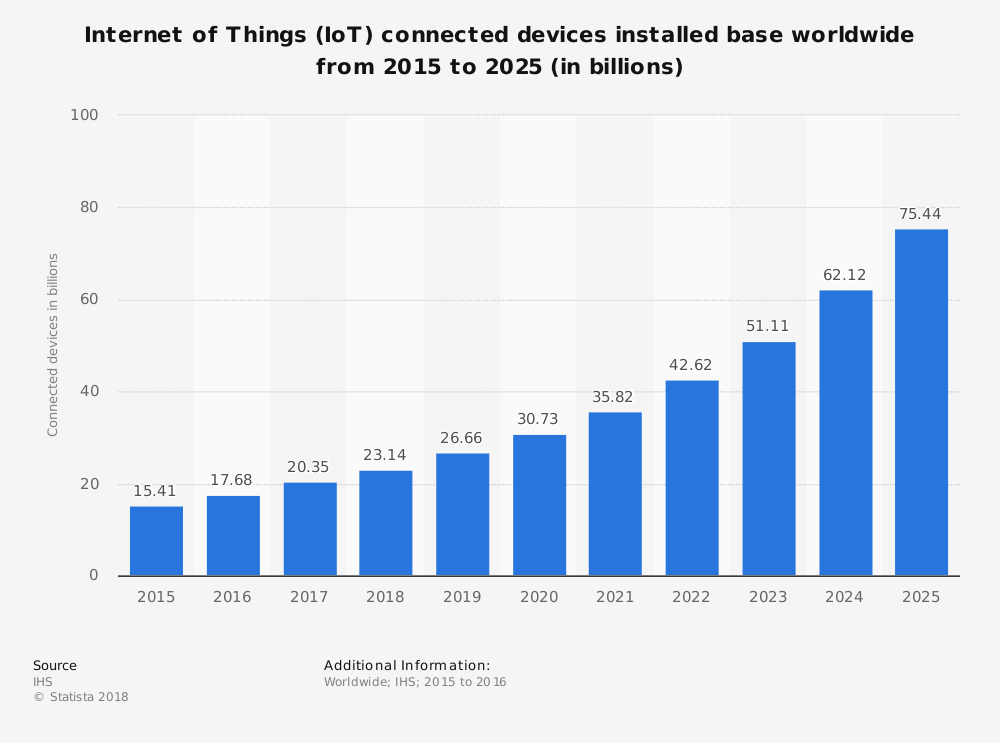
\includegraphics[width=150mm, scale=1]{Images/statista_iot.png}
      \caption{Statista: Predicted Growth in Online IoT Devices by 2025}
      \medskip
	  \small
		This graph is provided based on research by Statista Gmbh, showing their predicted growth trend for the number of internet-connected IoT devices by 2025. Historical data is included back to 2015.  
\label{fig:StatistaIoTPrediction}
\end{figure}

According to statistics published by Statista\footnote{Statista cite the original source of this data as being from IHS Markit, an analytics firm headquartered in London.} in 2018, \cite{StatisticIoTStatistics} by 2025 it is predicted that there will be over 75 billion IoT devices online globally: Several times greater than the human population of the world\footnote{The latest population statistics published by the Department of Economic and Social Affairs Population Division of the United Nations in 2017 \cite{UNWorldPopulation} estimate the population of the world at approximately 7.6 billion individuals.}\interfootnotelinepenalty=10000. Figure \ref{fig:StatistaIoTPrediction} shows their predicted exponential growth trend over the period from 2015. These devices include everything from environmental sensors to wearable technologies and process automation components, and are playing an increasingly important role in the lives of all members of society.  For a single IoT system, sensors could be used to collect information about a particular environment in a Wireless Sensor Network (WSN) configuration whilst communicating the information to a remote application, where it is aggregated and pushed to a set of distributed smartphones.


	
 \subsubsection{Security of IoT Devices}
Whilst connectivity between devices and processes has enhanced and optimised industrial processes, enabling the conception of countless new applications, the pace of this transformation has resulted in little to no attention being given to the security of these systems. Apart from concerns about the extent of pervasive monitoring conducted by IoT systems\footnote{The extent to which connected devices have become part of everyday life concerns many individuals, particularly since the primary purpose of IoT devices is to continuously gather, analyse and transport data to other systems. In an eye-opening paper published in 2017, \cite{7948540} Lackorzynski \textit{et al.} emphasise the dangers of internet-connected devices such as the \textit{Hello Barbie} childrens toy, which is ''a doll that could talk back to the user... in this case very probably a minor''. }, new applications are being found for IoT devices at such pace that instead of being built into these applications from the beginning, security is largely being left behind to catch up on later. Most of the time, it can be taken that there is no such thing as ''security by default''.

The risks - both to security and privacy - associated with the pervasiveness of the Internet in everyday life today are something that the general population are largely oblivious to. Insecam, which is a website broadcasting online feeds from thousands of IP cameras with default login credentials without the owners' knowledge, illustrates the gravity of this issue. \cite{Insecam} Devices and systems which never had communication capabilities before are being brought online, exposing them to significant potential tampering and misuse in ways that could affect the welfare of entire populations. Crucial systems on which society relies on a daily basis such as power grids, medical devices and traffic control systems are increasingly falling into this category, becoming exposed to attacks in a way that they never were in the past. 

Some of the greatest issues with the security of these devices include the following:

\begin{enumerate} \label{ReasonsForInsecureIoTDevices}
\item \textbf{Weak Default Credentials}

The main contributor to the success of most attacks on IoT devices  to date is the fact that these devices are shipped with weak default credentials that are identical across all instances of a given model. Additionally, these credentials are usually the only security measure used to mitigate against threats to these devices: There is very little effort required for an attacker to successfully compromise such a device.

\item \textbf{Limitations in Applying Updates}

The environments in which many IoT devices are deployed make it very difficult to patch vulnerabilities and apply updates to these devices. In general, large numbers of heterogeneous devices are deployed in a geographically dispersed, distributed setup and communicate over a variety of different networking protocols. Applying updates in such a deployment is inherently challenging.

\item \textbf{Limited Capacity for Encryption}

Due to the limited computational capacity and bandwidth of many low-powered IoT devices, the deployment of encryption on these devices is near to impossible. The compute-intensive operations required by most encryption protocols to both encrypt and decrypt data-in-transit and data-at-rest make it very difficult to implement encryption practically. To illustrate this, the Internet Engineering Task Force (IETF) stated in their most recent specification for Low-Powered Wide-Area Networks (LPWANs) that implementing key authentication mechanisms becomes ''challenging to handle in LPWANs with bounded bandwidth.'' \cite{ietf-lpwan-overview-10} As discussed by Dowling \textit{et al.}, if encryption is not implemented correctly, this can open the door for attacks on confidentiality, origin authentication and data integrity if the device in question is compromised. \cite{Dowling2017}

\item \textbf{Insecure Communication Protocols}

Many IoT devices use insecure communication protocols because of their requirement for low power consumption. The \textit{telnet} network protocol, which runs on port 23/TCP, has been largely retired as it is highly insecure, transmitting all traffic in clear-text including login credentials\footnote{The full telnet  protocol specification was finalised by the IETF 35 years ago in 1983, and explains the motivations behind the protocol and its intended uses. \cite{rfc854}}. It is however a lightweight protocol to deploy on a low-powered device, meaning that it has been widely included in IoT devices for authentication. This further weakens the security of these devices: A passive attacker eavesdropping on network traffic can capture IoT device data for later analysis or compromise the device itself.

\end{enumerate}

For attackers, IoT devices are very enticing: They are always online, using weak security mechanisms and often with access to powerful shells. The emergence of freely-available online scanning tools such as Shodan\footnote{Shodan is a search engine for internet-connected devices. If a search is performed for ''default password'', devices using default passwords are identified all over the world and returned to the user as a result. \cite{ShodanDefaultPasswordSearch}} mean that identifying these devices becomes trivial. As affirmed by leading cybersecurity expert Bruce Schneier in his article \textit{The Internet of Things is Wildly Insecure - And Often Unpatchable} in 2014, ''if we don't solve this soon, we're in for a security disaster as hackers figure out that it's easier to hack routers than computers''. \cite{TheresNoGoodWayToPatchTheIoT}

%% QUOTE SCHNEIER
\subsubsection{Internet of Things Botnets} \label{IoTBotnetsSoA}

Given the exponential growth in the number of internet-connected devices over the past several years, and given that attacks will always evolve as new technologies emerge,  new attack vectors and threats have been realised in relation to IoT devices since Bruce Schneier's insightful and telling article in 2014. \cite{TheresNoGoodWayToPatchTheIoT} Though many IoT devices are low-power devices commonly deployed in remote areas with low network bandwidth, large numbers of these devices can have a combined impact that packs a significant punch: Enter IoT botnets.

IoT botnets are likely the most active and topical breed of botnet at present. They are botnets composed entirely of compromised IoT devices. Most of these devices have been found to run the Secure SHell\footnote{The SSH protocol runs on port 22/TCP, and was designed by the IETF for secure remote login using encryption. \cite{rfc4252}} (SSH) and telnet authentication protocols with simple default username-password combinations, making it straight-forward to launch brute-force authentication attacks to gain root access to the device.

The highest profile attack to-date by an IoT botnet took the world by surprise in late 2016. The Mirai botnet, which amassed an army of over 300,000 IoT devices by capitalising on their poorly-implemented authentication mechanisms, conducted one of the biggest ever DDoS attacks by volume. The attacks began by targeting \textit{Krebs on Security}, \cite{KrebsOnSecurity} the website of well-known investigative security journalist Brian Krebs, eventually peaking at almost 1Tbps with an attack on French cloud hosting provider OVH. Research conducted by Antonakakis \textit{et al.} \cite{UnderstandingTheMiraiBotnet} on the success of Mirai found that for the 3 most common architectures found to be running the telnet protocol\footnote{MIPS 32-bit, ARM 32-bit, and x86 32-bit were the three most common CPU architectures identified in the collected device samples, accounting for circa 74\% of these. \cite{UnderstandingTheMiraiBotnet}}, ''security cameras, DVRs, and consumer routers represent(ed) the majority'' of these devices.

%\includewidefigure{UnderstandingTheMiraiBotnet_DefaultPasswordsTable}{The Mirai Botnet: Most Common Default Passwords}{A table provided in the \textit{Understanding the Mirai Botnet} paper, \cite{UnderstandingTheMiraiBotnet} showing the passwords that were most commonly found across all of the devices analysed in their research. }{Images/Understanding_the_Mirai_Botnet_-_table_of_default_passwords.png}

\begin{figure}[ht]
      \centering
      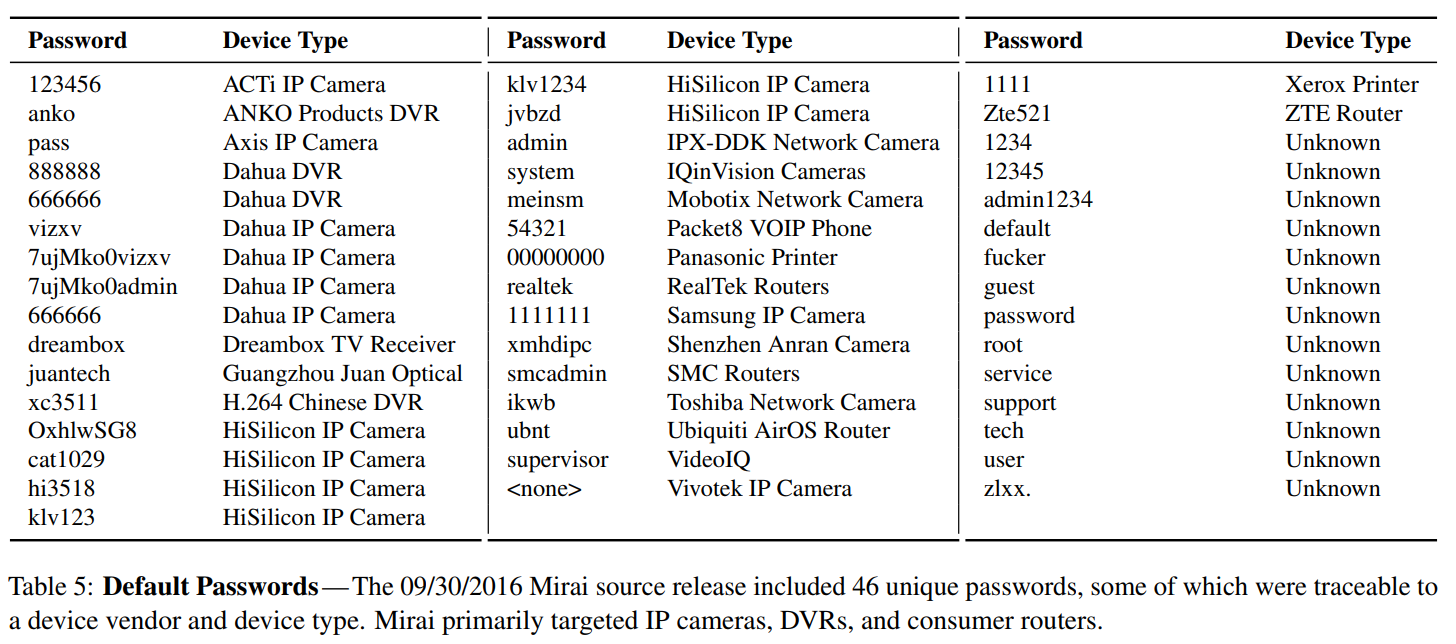
\includegraphics[width=175mm, scale=1]{Images/Understanding_the_Mirai_Botnet_-_table_of_default_passwords.png}
      \caption{The Mirai Botnet: Most Common Default Passwords}
      \medskip
	  \small
		A table provided in the \textit{Understanding the Mirai Botnet} paper, \cite{UnderstandingTheMiraiBotnet} showing the passwords that were most commonly found across all of the devices analysed in their research. 
\label{fig:UnderstandingTheMiraiBotnet_DefaultPasswordsTable}
\end{figure}

The scale and impact of this botnet was a revolutionary development. The fact that it was capable of threatening some of the worlds best-defended targets using enormous numbers of devices with low computational capabilities speaks volumes about the scale of issues that are currently being faced in IoT device security. As stated by Bruce Schneier in his 2017 article \textit{Botnet of Things}, ''botnets will get larger and more powerful simply because the number of vulnerable devices will go up by orders of magnitude over the next few years ... overall, the trends favor the attacker''. \cite{SchneierBotnetOfThings}

A number of other IoT botnets have surfaced since the Mirai attack, many of them variants of the original Mirai source code which was published online by a user called \textit{Anna Senpai} on the popular \textit{HackForums} site. \cite{WhoIsAnnaSenpaiKrebs} One noteworthy botnet is BrickerBot, an IoT botnet which surfaced shortly after the initial Mirai attacks on \textit{KrebsOnSecurity}. \cite{BrickerBotArticle} The author of this botnet, who calls themselves the \textit{janit0r}, claims to be a \textit{white hat}\footnote{This is a term commonly given to individuals who try to identify security vulnerabilities through hacking. They are different to malicious attackers in that they respect any relevant laws, and do not hack in order to damage the target system. Clearly, the \textit{janit0r} doesn't fit this description.} hacktivist intent on performing what they termed ''Internet Chemotherapy'': The complete destruction of IoT devices with poorly-implemented security measures as a punishment to their owners. In a farewell email made available to security site \textit{BleepingComputer} on 10th December 2017, the \textit{janit0r} warns that the world should ''WAKE UP TO THE FACT THAT THE INTERNET IS ONLY ONE OR TWO SERIOUS IOT EXPLOITS AWAY FROM BEING SEVERELY DISRUPTED'', and that organisations and individuals must take action to prevent this. \cite{janit0rFarewellEmail}


	
\subsection{Critical Service Infrastructures}
	
At a time where heightened political tensions exist between many of the world's most powerful nation states\footnote{The United States are currently locked in a cyber-combat against ''HIDDEN COBRA'', a codename for what they claim is North Korea's DDoS botnet infrastructure, as part of ongoing disputes between the two nations. A US national alert \cite{HiddenCobra} issued in June 2017 by the US-CERT claimed that HIDDEN COBRA had ''likely targeted the aerospace, telecommunications, and finance industries'' in the United States.}, cyber attacks are playing a prominent role in warfare and terrorism. Cyber attacks on critical service infrastructures have the potential to cause responses with severe impact.  Illustrating the severity of threats from competing nation states,  Unal \textit{et al.} \cite{NuclearReport2018} discuss the growing reliance of nuclear weaponry on digital technology and communication systems, stating that ''the likelihood of attempted cyber attacks on nuclear weapons systems is ... increasing from advanced persistent threats from states and non-state groups''.

In a report published in 2017 containing recommendations to the U.S. administration on national cyber-security, \cite{brenner_2017} M.I.T. researcher Joel Brenner states that one of the eight major challenges facing the United States government currently is to ''enable critical infrastructure operators to quickly identify and respond to cyber risk arising from cross-sector linkages as well as from their own network''. This statement encapsulates precisely the issues facing critical service providers worldwide today, and is something that is being reflected in incidents across the world with an increasing number of attacks on high-profile targets.

\subsubsection{Vulnerable Critical Infrastructures}
 It is clearer now than ever that key organisations and critical services require a renewed focus on defence strategies for their IT infrastructures. One such category of critical infrastructures is Supervisory Control and Data Acquisition (SCADA) systems, which are employed in industrial control environments to perform functions such as process control and monitoring. Typically, these systems deal with lots of components including sensors and mechanical parts like motors, enhancing the efficiency of operations in these environments. 
 
 Securing these systems is vitally important: They are the underlying control system of almost all nation-critical infrastructures such as transport, power and water. It is clear that the consequences of compromising these systems have the potential to be serious and far-reaching.

\subsubsection{Case Study: National Health Service Attacks 2017} \label{WannaCryNHSCase}
In May 2017, one of the more memorable attacks in recent years on a nation-critical service occurred in the United Kingdom. The global WannaCry \textit{ransomware} attacks, which successfully compromised more than 200,000 systems in over 100 countries, knocked systems in the UK National Health Service (NHS) at 37 sites offline for over a week with more than 6,912 appointments cancelled in that time. Though the NHS was almost certainly not a specific target of the ransomware authors\footnote{According to a paper published in the aftermath of the attacks, many other sectors across the world including transport and energy were also affected. \cite{MakingSenseOfRansomwareMess}}, the attacks had a huge impact on health services across the UK. \cite{AmyasMorseWannacry}

%\includewidefigure{NHS_WannaCry_Illustration}{Illustration of WannaCry Infection in the NHS}{An illustration of the infection of systems at NHS hospital sites by the WannaCry ransomware. The infection was not limited to user devices and servers, affecting systems including MRI scanners and blood test analysis devices. \cite{LessonsLearnedWannacryReport}}{Images/NHS_WannaCry.png}

\begin{figure}[ht]
      \centering
      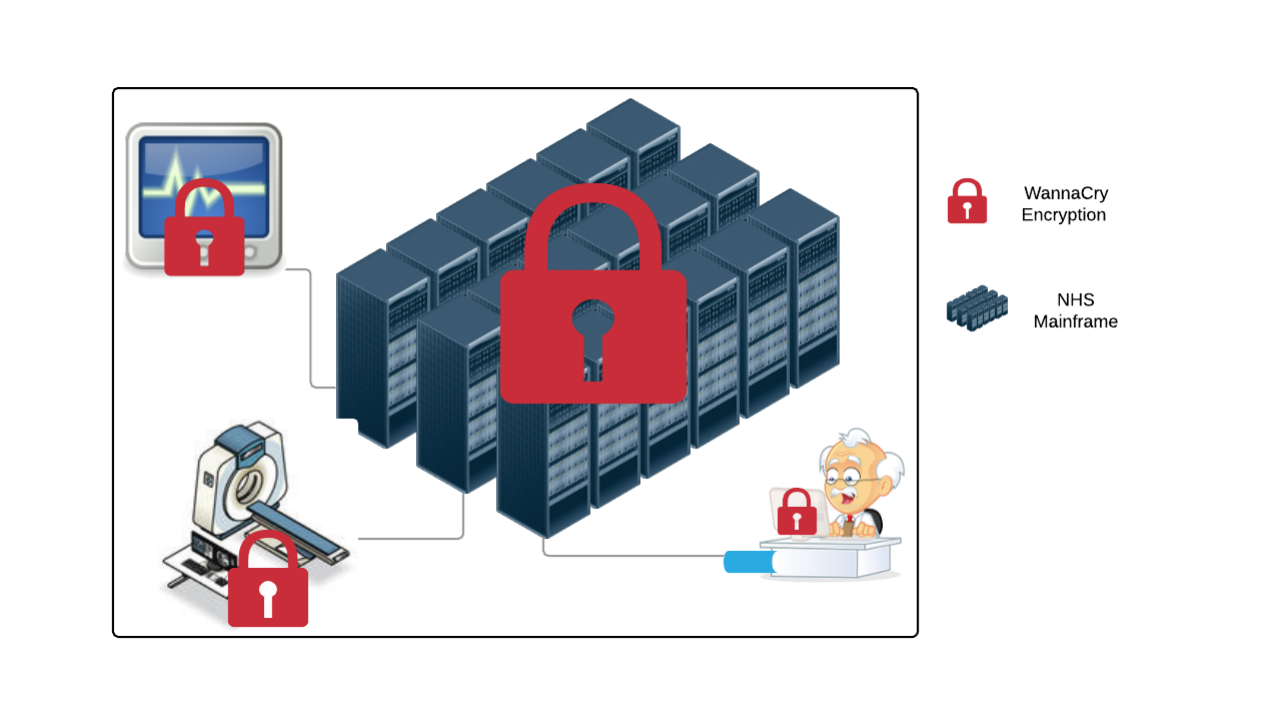
\includegraphics[width=150mm, scale=1]{Images/NHS_WannaCry.png}
      \caption{Illustration of WannaCry Infection in the NHS}
      \medskip
	  \small
		An illustration of the infection of systems at NHS hospital sites by the WannaCry ransomware. The infection was not limited to user devices and servers, affecting systems including MRI scanners and blood test analysis devices. \cite{LessonsLearnedWannacryReport}
\label{fig:NHS_WannaCry_Illustration}
\end{figure}

Examining the compromise of the NHS infrastructure by the WannaCry ransomware presents a strong basis for addressing many issues seen across critical service infrastructures. Being such a high-impact incident, it emphasises the severe consequences that a cyber attack can have on a critical service. An audit report published by the UK National Audit Office after the incident \cite{AmyasMorseWannacry} highlights a number of substantial shortcomings in the NHS security defence strategies up to 12th May 2017 when the attacks occurred:
	
	\begin{enumerate}
		
		\item There was no incident monitoring in place to alert security first-responders to any unusual behaviour in the NHS systems: Evident from the fact that it took over half a day to reach those who could take remedial action. 
		
		\item There was no centralisation of system data, meaning that security experts had to physically attend the affected sites in order to collect crucial data about the attacks. This further prolonged the period for which these systems remained inoperable. 
	
		\item Prior to the incident, recommendations regarding  updates for the NHS IT systems were issued but not followed at the affected sites. Further to this, there was no system in place to determine whether or not the actions had ever been taken. Outdated and unpatched operating systems were a major contributor to the success of the compromise, which was entirely based on a Windows exploit\footnote{WannaCry and NotPetya, two ransomware strains which made their first appearance in 2017, both exploited this vulnerability. Officially named 'EternalBlue MS17-010' by Microsoft, a patch was released for it after major attacks by both of these ransomware strains. According to an article by Brian Krebs, \cite{KrebsWannaCry} The EternalBlue vulnerability exploits the Microsoft Server Message Block (SMB) network file sharing protocol. SMB allows applications on a computer to read and write to files and to request services that are on the same network.}.	
	\end{enumerate}
	
	% How did it happen exactly? A trusted node on the outskirts of the network (such as a GP) received the infection, and it was propagated back into the NHS mainframe where is was able to root itself and spread to other parts of the network.
    
    Ultimately, the lack of monitoring within the NHS systems meant that when the attacks occurred, the systems at the affected sites remained offline for an extended period of time, causing chaos across the entire healthcare system in the UK.  It is clear that in order to protect both their own systems and those of others that depend on them, organisations must place emphasis on security training for their members, the security and maintenance of their technologies, and the rigorousness of governance of their systems. 




%%
%%	Section 2: Intrusion Detection Technologies
%%
%%


\section{Intrusion Detection} \label{IntrusionDetectionSection}

An Intrusion Detection System (IDS) is a security application that is employed to detect attempts from an attacker to gain unauthorised access to a system or system resource. They are usually deployed in a region known as the De-Militarised Zone (DMZ), a sub-network separating an internal network from untrusted external networks, providing an added layer of isolation between internal and external systems\footnote{Usually, content-serving systems are placed in this region of the network so that they can be accessed from external networks.}. Most traditional IDSs work off the basis of comparing activities to a defined security policy, and either permitting or denying the action on this basis.

In this section, the motivations for intrusion detection, along with two primary types of intrusion detection system, are discussed and compared.


\subsection{Motivations for Intrusion Detection} \label{MotivationsForIntrusionDetection}
IDSs play an important role in securing both enterprise and personal systems. Among the many advantages are the following:
\begin{itemize}
\item By detecting an intrusion in the early stages, the intruder can be removed from the system before any damage is done.
\item Attackers in general strive to remain anonymous and undetected. If a potential intruder has some knowledge of an effective IDS being in place in a system, they may be deterred from proceeding with an attack.
\item Valuable information may be collected about the nature of the intrusions and how they took place, enabling administrators to continuously re-evaluate their system design and security strategies. 
\end{itemize}

How each of these advantages are provided, and to what extent, is dependent on the type of IDS being employed. It should be recognised that threats can come from nodes both internal and external to the network in question, and so a maximally effective IDS will address both. 

IDSs can be broadly categorised as either being \textit{passive} or \textit{active}.
\begin{itemize}
\item Passive IDSs are not proactive about preventing or interfering with attacker activities.
\item Active IDSs are proactive about engaging with the attacker in order to counter an attack.
\end{itemize}


In this section, two particular IDSs will be discussed in detail: firewalls and honeypots.


\subsection{Firewalls}

Firewalls are the most commonly deployed type of IDS, and are used in virtually all enterprise networks as part of an organisation's network security. In general, they are classified as a \textit{passive network defence mechanism}. According to a literature survey by Voronkov \textit{et al.}, "a firewall is a system consisting of software and/or hardware that is designed to prevent unauthorized access to/from a network or device". \cite{Voronkov:2017:SLR:3161158.3130876}



\subsubsection{Overview}
The basic principle of operation of a firewall is to act as a barrier on the periphery of a network, preventing intruders and malicious forces from gaining access  to the system being protected. In practical terms, they filter network packets based on a defined security policy which is a set of configured rules, and either accept or reject a given packet according to this policy.


%\includewidefigure{Firewall_DMZ_Illustration}{Use of Firewalls in a De-Militarised Zone}{An illustration of a typical corporation network where firewalls have been employed at the internal and external entrypoints to the De-Militarised Zone (DMZ).}{Images/Illustration_of_Firewalls_in_a_DMZ.png}

\begin{figure}[ht]
      \centering
      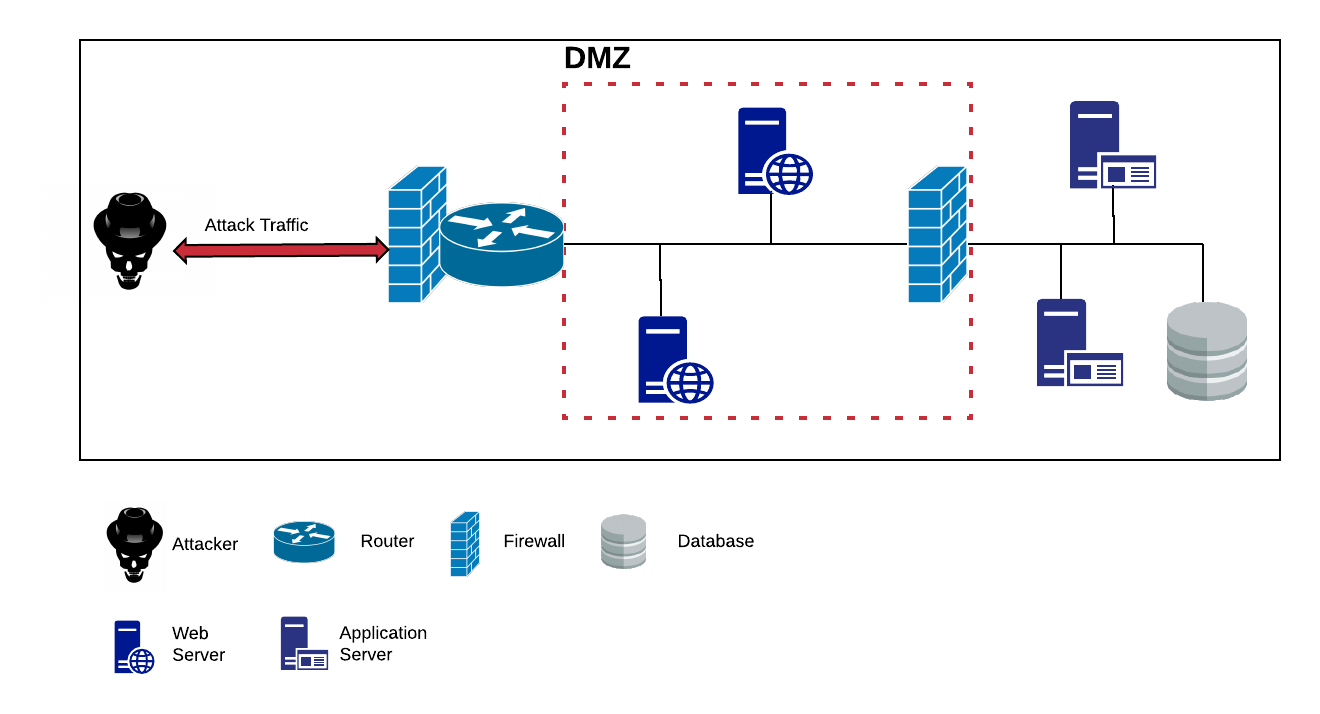
\includegraphics[width=175mm, scale=1]{Images/Illustration_of_Firewalls_in_a_DMZ.png}
      \caption{Use of Firewalls in a De-Militarised Zone}
      \medskip
	  \small
		An illustration of a typical corporation network where firewalls have been employed at the internal and external entrypoints to the De-Militarised Zone (DMZ).
\label{fig:Firewall_DMZ_Illustration}
\end{figure}

\subsubsection{Design}
A number of commonly employed approaches to implementing firewall policies are identified by Omar Santos in \textit{End-to-End Network Security defence-in-Depth}. \cite{OmarSantos} Some of these are described as follows:

\begin{itemize}
\item \textbf{Pattern Matching}

The firewall tool searches for a fixed sequence of bytes within a packet, often aligned at a specific position corresponding to a field within the packet. It then makes a filtering decision by consulting its defined security policy.

One of the primary limitations of pattern matching is that it generally exhibits a high rate of false positives, making it relatively inaccurate as a technique of classifying packets that should be denied access. 
\item \textbf{Protocol Analysis}

Protocol analysis is accomplished by decoding protocol-specific communications, i.e. by examining the packets corresponding to particular communication protocols. The firewall will identify elements of the protocol and examine them for an infringement, for instance by examining explicit fields within the packets. An example for an SMTP packet might be examination of fields such as \textit{HELO}, \textit{MAIL}, \textit{RCPT}, \textit{DATA}, \textit{SET}, \textit{NOOP}, and \textit{QUIT}.
\item \textbf{Heuristic-Based Analysis}

Also known as \textit{misuse detection}, this technique tries to identify intruders based on a set of known undesirable behaviours and patterns that can be determined according to rules. Systems built upon this concept are severely limited in intrusion detection capabilities since they cannot detect an intrusion for which no rule is defined. 

\item \textbf{Anomaly-Based Analysis}

Anomaly-based analysis techniques try to define the behaviour of a normal user over time, and compare the behaviour of all users to this in order to identify suspicious behaviour that may relate to an intrusion. 

\item \textbf{Deep-Packet Inspection}
 
Deep-Packet Inspection (DPI) involves closely examining information embedded in network packets in order to make more informed decisions about how to handle the packet. This often allows for more effective mitigation against attacks such as DDoS, where DPI allows for the more accurate identification of packets that have undesirable contents or are in some way not legitimate.

\end{itemize}


\subsubsection{Challenges} \label{ChallengesForFirewalls}

% 

% Passive security mechanisms in general are notoriously hard to deploy, e.g. IPSEC, DNSSEC, etc. Firewalls are no different: They are very restrictive for the normal use and operation of the system they are deployed in, and so are often configured incorrectly or ineffectively in order to facilitate usability.

There are a number of issues with using firewalls alone for intrusion detection. Though at a point in time these systems reflected the configuration of enterprise networks accurately, in the world of the modern web many of the premises of using firewalls simply do not hold any more. As enumerated by Steven M. Bellovin in \textit{Thinking Security: Stopping Next Year's Hackers}, \cite{ThinkingSecurityBellovin} the design and use of firewalls is based on the following premises:


\begin{enumerate}
\item A firewall operates at a \textit{topological chokepoint} in the network it is protecting, such that it partitions two sections of the network.
\item All nodes being protected inside the firewall have the same security policy.
\item All nodes inside the firewall are trusted.
\end{enumerate}

If all of these conditions hold, then a firewall will work well in the system in question. However, taking any modern IT infrastructure in an organisation today, most - if any - of these assumptions do not hold true. 
\begin{itemize}
\item Enterprise networks increasingly deal with nomadic users, who are facilitated in constantly connecting to and disconnecting from these networks without any security auditing being performed.
\item The devices that connect to enterprise networks today are incredibly diverse, and implement an even more diverse and inconsistent range of security policies.  
\end{itemize}

On top of this, it is increasingly becoming difficult for firewalls to use packet inspection techniques to filter network traffic because of incompatibility with other security mechanisms. An increased uptake in TLS encryption and the push for packet header encryption is causing enormous issues for the operation of firewalls, which cannot decrypt packets in order to make the required filtering decisions that it depends on.

There is no question that firewalls are no longer sufficient on their own in providing security for modern networks. They can be reasonably effective against known, less sophisticated attacks and are less effective against more sophisticated targeted attacks which are more likely to use new exploits. As Fred Schneider explains in his paper \textit{Blueprint for a Science of Cybersecurity}, ''a secure system must defend against all possible attacks - including those unknown to the defender. But defenders, having limited resources, typically develop defences only for attacks they know about.'' \cite{Schneider11_BlueprintForScienceOfCybersecurity}

Overall, firewalls are most effective when used in combination with other security mechanisms, but their inability to classify and mitigate against new threats is a major limitation to their use. \cite{ThinkingSecurityBellovin}

%% Could also talk  about the limitations of using firewalls, since it is far more likely that a legitimate user will be identified as an intruder: Pessimistic assumption that the user is more likely to be an attacker than a harmless user.


\subsection{Honeypots} \label{HoneypotsSection}

%% Deception is the primary underlying principle behind the use and design of honeypots: They serve as a deterrent, since an attacker may waste valuable time pursuing misleading information instead of achieving their goals.


Well-known security expert and Honeynet Project founder Lance Spitzner defines honeypots as "a security resource who's value lies in being probed, attacked or compromised". Honeypots leverage the concept of deception in order to combat attackers. As explained in a paper by Cliff \textit{et al.}, ''the essential parts in cyber deception include crafted information by the defender (that will be used to mislead) and wrong actions taken by the adversary as a result of the deception.'' \cite{8328971}

Put simply, honeypots are devices which masquerade as legitimate and systems in order to detect, track and analyse patterns of user behaviour when the system is illegally accessed. They are categorised as an \textit{active network defence mechanism}, and are deployed solely with the intention that they will be attacked.  A key characteristic of a successful honeypot is attractiveness to an attacker. 'Attractive' in this context means that the honeypot should appear to be exactly the device that the attacker is looking for: A device that has the potential to be easily exploited, whilst offering maximum value to the attacker. 

%% Honeypots try to make it more difficult for an attacker to gain anything from attacking a network.
%% Honeypots work off the principle of deception.

\subsubsection{Overview}

Honeypots are broadly seen as acting as both decoys and sensors in the network in which they are deployed.

\begin{itemize}
\item \textbf{Honeypots as Decoys}

A honeypot can be used to divert an attacker's attention away from the valuable components of the network in which it is deployed. This is particularly useful in a production environment, when there is a need to protect important systems on the network. 

In order for this strategy to be effective, the honeypot should appear to be exactly what the attacker is looking for. By then being attacked, the honeypot can immediately notify system administrators of an intruder being present in the network, allowing them to take the appropriate course of action to secure it.

\item \textbf{Honeypots as Sensors}

Honeypots can also be viewed as sensors, since they can collect valuable data about the attacks that they receive. This is particularly useful for detecting weaknesses and vulnerabilities in system design, since the captured attack data can be analysed to understand the attacker's behaviour and strategies as well as their motivations.
\end{itemize}

Thus, the value of honeypots is both in their ability to capture information as well as to defend the system within which they are deployed.

Amongst the many benefits of using honeypot technologies are the following:

\begin{enumerate}
\item \textbf{Configurability}

In general, honeypots are highly configurable and customisable and can be made to mimic real systems. This configurability allows those deploying them to adapt their defence strategy to tackle evolving attack behaviours.

\item \textbf{Inside the Network} 

Honeypots are deployed inside the infrastructure of the system they are protecting, rather than on the fringes as with firewalls. This allows for security much closer to the real systems that are being targeted by attackers.

\item  \textbf{Logging Capabilities} 

Honeypots give a unique opportunity to capture valuable information about the nature of attacks being launched against a system, providing a means of observing attackers 'in the wild' without being detected. This gives system administrators a better chance of staying up-to-date with the evolving security requirements of their systems.

\item  \textbf{Few False Positives}

The premise of using a honeypot is that nobody should communicate with it: There is no legitimate reason to interact with a honeypot, since it is deployed with the sole purpose of attracting attacks. This means that typically, a honeypot will trigger very few false positives, since every interaction with a honeypot is automatically distrusted. This has added benefits for system administrators in that there is a lesser requirement to comb through very large log files in order to identify a significant event, which is common practice with firewalls and many other IDSs.

It is important to consider however that individuals within an organisation may mistakenly interact with the honeypot out of curiosity, something which can often be deduced from looking at the logging captured. In general, the presence of honeypots in a system should not be well-known within the organisation for this reason.

\item  \textbf{Offensive and Defensive}

As explained, honeypots are an active defence mechanism. They allow for learning about adversarial intent, capability, and techniques as well as thwarting attempts to compromise real systems. By using honeypots, cyber attacks can be mitigated against by making access to valuable systems both expensive and ineffective.
\end{enumerate}


\subsubsection{Design} \label{HoneypotDesignSoA}
The design of honeypots to suit the context of their deployment is key to their ability to provide effective intrusion detection in a system. The primary design categorisations of honeypots were outlined in a paper by Mokube \textit{et al.} \cite{Mokube:2007:HCA:1233341.1233399} on the basis of (i) their level of interactivity with an attacker, and (ii) the context of their deployment.

\paragraph{Interactivity} \label{HoneypotInteractivityLevels} \mbox{}\\ 
Interactivity levels of honeypots are an important consideration, which define (i) the ability of the attacker to interact with the honeypot, and consequently (ii) the volume and type of information that can be gathered by that honeypot. Levels of interaction range from simply allowing a connection to be made, to being able to download and install malware binaries. The cost versus learning benefits of honeypot interactivity levels increase proportionally, meaning that a highly interactive honeypot will likely be expensive to host and maintain. 

Any effective honeypot must be capable of interacting at some level with an attacker, while also quietly monitoring their actions. There are three practical classifications of honeypot interactivity level: Low, high and medium.

\begin{itemize}
	\item \textbf{Low}
	
	Low-interaction honeypots are most commonly used to alert someone to the fact that an attack has occurred, but do not provide any means of interacting with the attacker or capturing the attack data. They are used in cases where a lower-risk solution is preferred: In general, a low-interaction honeypot will simply be an emulation of a real service, and so does not offer any opportunity for system compromise by an attacker. This can be a major limitation to their use, since there is very little knowledge to be gained from preventing further interaction with an attacker.
	
	\item \textbf{High}
	
	High-interaction honeypots are at the other end of the spectrum compared to low interaction honeypots. They are fully-fledged systems, and give the opportunity for attackers to use real applications during their interactions. A great deal can be learned about the nature of attacks from using high-interaction honeypots, since it is the closest thing to observing attacks ''in the wild''. The trade-off is the high-risk associated with the exposure of a real device to a malicious attacker, which in the worst case could see the entire system taken over by an attacker and used to launch further attacks on other devices. Some of the ethical considerations around this issue are discussed in \textit{Section \ref{EthicsOfHoneypots}.}
	
	\item \textbf{Medium}
	
	As described, the appropriate level of interactivity of a honeypot depends on the use context: Low-interaction devices are commonly used for detecting connection attempts, whereas high-interaction devices are live systems that can capture detailed information about the behaviour of attackers ''in the wild''. Medium interaction honeypots offer a good middle-ground, using emulated components of a real system to allow a level of interactivity with the attacker whilst not exposing any real systems that could be compromised.
	
\end{itemize}

A summary of the characteristics of each of these categories of honeypot are given in table~\ref{table:honeypot-interaction}.

\begin{table}[!h]
	\begin{center}
		\begin{tabular}{|c|c|c|c|} 
			\hline
			\bf Interaction Level  & \bf Information Quality  & \bf Risk  & \bf Maintenance Cost \\
			\hline
			High & Excellent & High & Difficult  \\
			Low & Poor & Low & Simple \\
			Medium & Good & Medium & Relatively Simple \\
			\hline
		\end{tabular}
	\end{center}
	\caption[Comparison of Interaction Levels of Honeypots.]{A summary of the characteristics of each different honeypot interactivity level, similar to that provided in a survey of honeypot technologies by Nawrocki \textit{et al.}. \cite{Nawrocki2016} In general, the higher the interaction level the higher the cost, risk and value of information captured.}	
	\label{table:honeypot-interaction}
\end{table}

\paragraph{Deployment Scenarios}

There are primarily two deployment scenarios for honeypots: Production and research. This distinction mainly distinguishes between the function that the honeypot needs to provide for the system in which it is to be deployed.

\begin{itemize}
	\item \textbf{Production Honeypots}
	
	Production honeypots are generally deployed in large, enterprise networks with the intention that they will act as a part of the active network defence in the organisation's infrastructure. An example of such a deployment is shown in figure~\ref{fig:Honeypot_DMZ_Illustration}. Their primary purpose is to act as a decoy, luring the attacker away from valuable machines on the network with a seemingly more valuable and vulnerable target. This enables the honeypot to alert system administrators early on to the fact that there has been an intrusion, giving them the opportunity to isolate the valuable devices in the network from the infected honeypot. As previously highlighted, it also enables system administrators to identify vulnerable points in their infrastructure.


%\includewidefigure{Honeypot_DMZ_Illustration}{Use of Honeypots in a De-Militarised Zone}{An illustration of a typical corporation network where honeypots have been employed in conjunction with internal and external firewalls, inside the DMZ.}{Images/Illustration_of_Honeypots_with_Firewalls_in_a_DMZ.png}

\begin{figure}[ht]
      \centering
      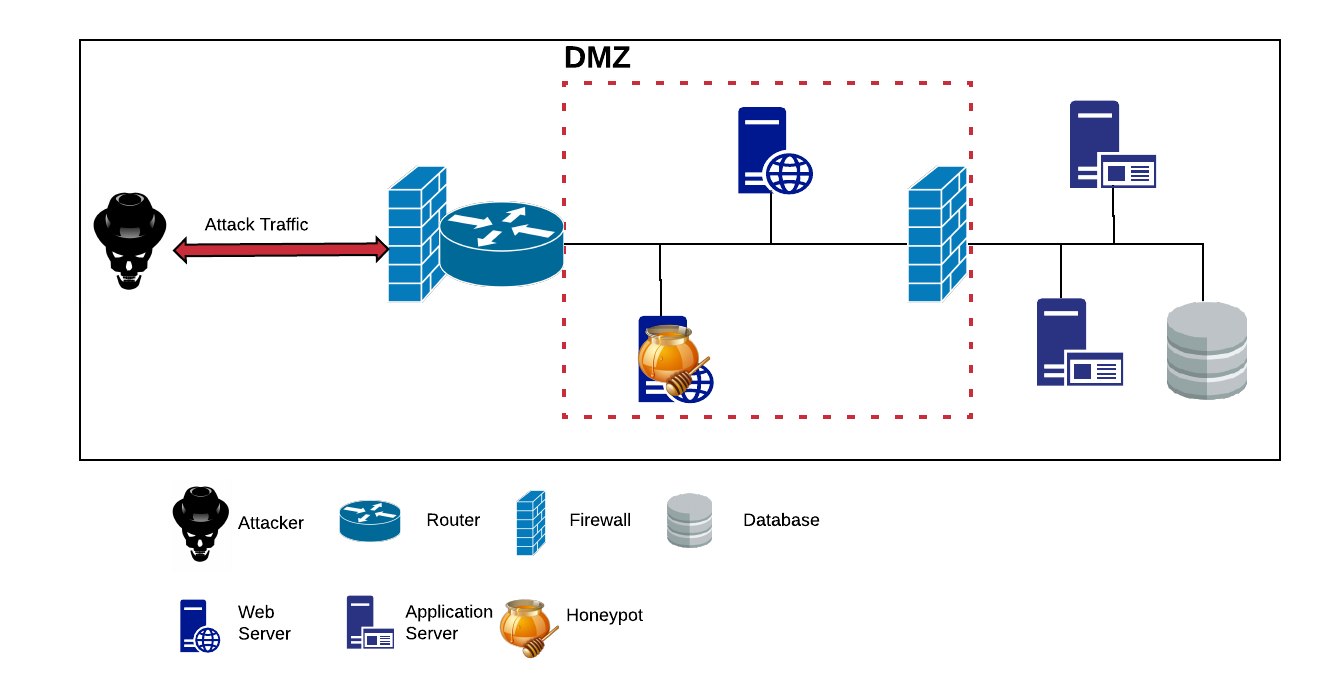
\includegraphics[width=160mm, scale=1]{Images/Illustration_of_Honeypots_with_Firewalls_in_a_DMZ.png}
      \caption{Use of Honeypots in a De-Militarised Zone}
      \medskip
	  \small
		An illustration of a typical corporation network where honeypots have been employed in conjunction with internal and external firewalls, inside the DMZ.
\label{fig:Honeypot_DMZ_Illustration}
\end{figure}
    
	The idea of attracting attackers into the system, encouraging them to interact with it and give away their attack strategies without causing any harm to the systems with real production value is the major attraction of using honeypots in a production environment. 
	
	
	\item \textbf{Research Honeypots}
	
	As the name suggests, these honeypots are generally deployed for the purpose of research rather than as a security measure. The emphasis with these honeypots is not so much on the ability of the honeypot to act as a decoy, and more on the ability of the honeypot to collect valuable data for analysis. By allowing attackers to interact with and infect the honeypot, research can be carried out relating to the behaviour and strategies of the attackers.
	
\end{itemize}

\subsubsection{Comparison with Firewalls}

When compared to traditional, passive intrusion-detection mechanisms such as firewalls, honeypots exhibit some crucial differences. 

\begin{itemize}
\item Firewalls define all attackers passively and simply alert to the fact that a security incident, such as an unauthorised connection attempt, has occurred. A system administrator can then, for instance, blacklist\footnote{Blacklisting an IP address means that it is added to a list of addresses that aren't considered trustworthy.} the source IP address of the connection to deny it access to the system. 

However, if a new attack comes along for which there is no rule defined in the firewall's security policy, the firewall is not able to deal with this attack. This illustrates how firewalls can only provide \textit{known-threat mitigation}.
\item In contrast to firewalls, honeypots proactively entice attackers to give away their attack strategies and intentions by leaving their tracks behind on the device. This enables the same system administrator to do far more to enhance their system security policies and identify potential flaws in their infrastructure, allowing them to \textit{improve} their system's security. 

As well as this, the honeypot can attract and deal with previously \textit{unknown threats}, giving them another edge over firewalls since they can provide \textit{unknown-threat mitigation} as well as \textit{known-threat mitigation}.
\end{itemize}

By using honeypots, system administrators are able to learn what attackers are targeting in their systems, enabling more effective defences to be implemented as vulnerabilities and flaws are identified. As suggested by Bellovin, ''the world has changed ... the decision to rely on (firewalls) should be reexamined and perhaps abandoned''. Despite this, firewalls are not obsolete and will continue to play an important role in IT and network security with their ability to detect and classify potential security risks at the edge of the network they are protecting. They are however best used in conjunction with active network defence mechanisms such as honeypots. \cite{ThinkingSecurityBellovin}


\subsubsection{Honeynets} \label{HoneynetsExplanationSoA}
%% Describe honeynets and how they can be beneficial as part of the network security of a system.
Honeynets are networks of interconnected honeypots, which coordinate their efforts to provide active network defence. Given that they consist of more than one honeypot, they have additional abilities to capture valuable attack information regarding threats compared to standalone honeypots: For instance, it is possible to study the propagation of attacks from one honeypot to the next, and to simulate a variety of different systems that may attract different categories of attack.

Honeynets are significantly more complex than standalone honeypots given that they consist of a network of honeypot devices designed to be attacked. In general, a honeynet will contain \textit{high interaction} honeypots so that an attack is able to propagate from one real system to another real system. As with individual honeypots, any connections to a system in the honeynet are immediately distrusted and assumed to be malicious. 

An element of a honeynet which is described by Lance Spitzner in \textit{Honeypots: Catching the Insider Threat} \cite{Spitzner:2003:HCI:956415.956438} is something that he refers to as the \textit{honeywall gateway}, a bridging device between external systems and the honeynet. All traffic between the external system and the honeynet must pass through this gateway. The honeywall will typically have two interfaces: One to connect it to the external web, and the other to connect to the honeynet. The honeywall thus acts to separate the honeynet from the external web. Since the honeynet is only reachable through the honeywall, which can monitor and control network traffic to and from the honeypots in the network, extensive extra monitoring can be performed on attackers of the system. Depending on the configuration, this component has the opportunity to capture data including network traffic and keylogging data.

\begin{figure}[ht]
      \centering
      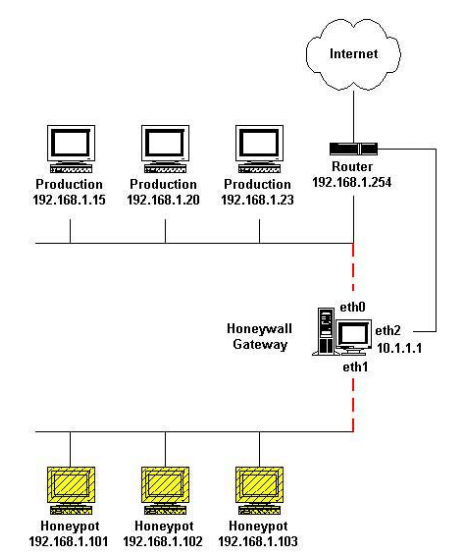
\includegraphics[width=100mm, scale=0.6]{Images/honey-wall-without-meta-data.png}
      \caption{Lance Spitzner's Proposed Honeynet Architecture}
      \medskip
	  \small
		This figure shows a diagram taken from Lance Spitzners paper proposing a honeynet architecture. Original source: \textit{Honeypots: Catching the Insider Threat}. \cite{Spitzner:2003:HCI:956415.956438}     
\end{figure}

% ^.
In summary, using a honeynet allows for deployment of a highly-controlled active defence network where all activities of attackers are made visible. The insights that can be gained from observing the behaviour of attackers in an unrestricted networked environment are highly valuable to those who wish to continuously improve their system defences. However, the risk associated with hosting a system of this type is a major trade-off since there are many more points of failure in a network of intentionally vulnerable devices.


%\subsubsection{Honeypots for Botnet Analysis}
%Honeypots have been widely used in the study of botnets and other categories of attacker.
%They provide researchers and reverse engineers with a platform to analyse both infection and operation of malware. Botnets are just a subset of this malware, where it is interesting and useful to study the operation of the malware as it is executing. High interaction honeypots thus seem to be a great solution for this problem.

\subsubsection{Challenges} \label{HoneypotSoAChallenges}
There are a number of challenges to the widespread deployment of honeypots in networks, outlined below.
	\begin{enumerate}
    
    \item {\textbf{Detection}}
    
	One of the major considerations when designing or using a honeypot-driven solution is the risk of the honeypot being detected as a non-genuine system. This is particularly relevant to low and medium-interaction honeypots which emulate a real system: It is never possible to exactly mimic the behaviour of the corresponding real system. This means that carefully crafted actions by an attacker may allow them to detect that they are not interacting with a bona-fide system by triggering different responses: A form of fingerprinting. It is an ongoing challenge for honeypot designers to combat fingerprinting checks by attackers.
    
    In general, honeynets are less likely to be fingerprinted successfully than an individual honeypot since they provide a network of interconnected high-interaction honeypots providing real services. This kind of system is highly enticing to attackers because of the advanced system capabilities that it provides, and thus a less likely suspect as a non-genuine system.

	\item{\textbf{Adoption}}
    
	There are many challenges to overcome in order to make the use of honeypots more widespread. To many, the idea of inviting a malicious actor into a production system seems like a potentially destructive action, and so many system administrators do not consider honeypots as part of their security infrastructure. Canary, a honeypot solution developed by Thinkst Applied Research, highlight on their product landing page the challenge behind adopting honeypots in large networks: ''With all the network problems we have, nobody needs one more machine to administer and worry about''. \cite{CanaryThinkst} Although it could be argued that this is a sales pitch, this statement highlights the demand and lack of supply of feasible solutions for large organisations regarding deployment and maintenance of honeypot-based systems. 
	
	\item{\textbf{Ethical Concerns}}
    
 	The use of any surveillance technology, which is the category into which honeypots fall, has ethical questions associated with it. Honeypots are widely accepted as an ethical approach to intrusion detection and understanding cyber attacks. Since there is no legitimate reason for interacting with a honeypot, any interactions are likely to be of a malicious nature - in which case, the honeypot simply serves to counteract further attacks of this type in the	future. Mokube \textit{et al.} discuss these ethical issues in detail in their paper. \cite{Mokube:2007:HCA:1233341.1233399} However, a discussion in a whitepaper published by the System Administration, Networking, and Security Institute (SANS), \cite{SANSPreemptiveDeterrence} it can be concluded that their use does not involve:
 	
 	\begin{itemize}

 		\item Entrapment, since there is no inducement to attack the honeypot - rather, it is something that all devices are vulnerable to because attackers will always seek to attack devices within their reach, regardless of whether it may be a honeypot. As aptly phrased by security researcher Lance Spitzner \cite{HoneypotsAreTheyIllegalSpitzner}, ''attackers find and break into honeypots on their own initiative''.
 	
 		\item Invasion of privacy, since surveillance mechanisms are broadly seen to be acceptable where they serve simply to protect their own environment. A commonly encountered example in physical environments is the use of CCTV cameras.
 		
	\end{itemize}

		Overall, the ethical concerns around the use of honeypots are widely accepted to be resolved by the nature of the deployment of honeypots: Ultimately, their purpose is to defend against unethical actions by attackers. With reference to the research being undertaken in this project, ethical considerations are discussed later in relation to the design of the research environment in \textit{Section \ref{EthicsOfHoneypots}}.
\end{enumerate}

\subsection{Cyber-Incident Monitoring}
Cyber-incident monitoring forms an important part of providing effective intrusion detection. Cyber incident monitors are platforms that support system administrators in identifying and acting upon threat intelligence collected through intrusion detection mechanisms such as honeypots and firewalls, primarily through providing enhanced usability and more effective communication. It is concerned with the effective management of intrusion detection tools, the recording of threat events, and the provision and presentation of threat information to first-responders. 

 %adding visual aids to the interpretation of honeypot data is a key element to bringing security into container-based architectures.

\subsubsection{Usability in Security}
It is widely accepted that the ability of a user to easily employ security systems makes a crucial contribution to their effectiveness: As argued by Sasse \textit{et al.}, ''security mechanisms are often too time consuming for people to bother with, or so complex that even those willing to use them make mistakes.'' \cite{7676149} The use of security mechanisms adds an overhead to the use of systems almost without exception. Apart from the consequent disincentive for individuals to use these mechanisms, it becomes very hard to use them effectively when their use is not straight-forward.

In a literature review addressing the usability of firewall applications in particular, Voronkov \textit{et al.} found that usability studies could greatly enhance the effectiveness of security mechanisms, since configuring them ''is a process that is complicated and prone to error...  misconfiguration of firewalls leads to a broad number of vulnerabilities in the network; environments with distributed and multiple firewalls just make matters worse.'' \cite{Voronkov:2017:SLR:3161158.3130876}

\subsubsection{Visualisation in Security}
Visualisation techniques have become crucially important in delivering usable security solutions. Security problems are inherently complex: In the case of tools such as firewalls which work off the basis of a list of defined rules, it becomes very difficult to understand and maintain the overall security policy as the list grows.

The impact of using visualisation in security mechanisms is that threat intelligence is communicated more clearly and effectively to those consuming the data. Ease of visibility of the state of a system is a crucial element of active network defence in identifying and investigating potentially malicious activities and detecting unknown threats before they can do damage. As explained by Vasilomanolakis \textit{et al.} in a paper detailing the development of a honeypot-based incident monitoring system, such a system ''unif(ies) the various alert generators into a single system that assists the user to make informed decisions''. \cite{Vasilomanolakis}



%%
%% 	SECTION 3: Modern System Infrastructures 
%%
\section{Modern System Infrastructures} \label{ModernSystemsInfrastructures}
There is a significant shift in the hosting solutions that are being used by large organisations that rely heavily on their IT infrastructure, particularly for those providing services on such a platform. Outsourcing of resource management is now the preferred approach for many large organisations, given that specialised hosting providers are increasingly offering end-to-end solutions for hardware, network and security infrastructure management.

The architectural design of these distributed services is also evolving. The concept of decoupling services by deploying them as microservices has enhanced operational efficiency in organisations, moving away from failure-prone monolithic designs of the past.

\subsection{Infrastructure-as-a-Service} \label{IaaS}

In the past, organisations hosted their systems on servers and physical infrastructure that they owned and managed themselves. This approach was resource-intensive for organisations, motivating the development of IaaS. IaaS is a service model where physical infrastructure is provided to organisations on an outsourced basis including hardware, storage, servers, data centre space and network components, and the use of cloud platforms which allow an organisation to host their services on another organisation's hardware offers a practical solution to this. 

\subsubsection{Benefits} 
The benefits for organisations of outsourcing their infrastructure management to third-party providers include the following:

\begin{itemize}
	\item  There is a guarantee of maximum uptime since cloud platforms are a paid service.
	\item There is no need for upfront capital investment, since there are none of the installation or maintenance costs associated with hardware upgrades or expansion.
	\item There are a wide range of geographic locations available for deployment since hosting services are located all over the world, allowing organisations to host their services closer to users that are geographically dispersed.
\end{itemize}

In essence, using a cloud platform to host enterprise-level systems is highly economical, simplifying the management of resources and deployment with the result that they consume less of the focus of system administrators. With an ever-increasing number of companies moving their operations to the cloud, a cloud-deployment appears to be the most feasible deployment solution for cyber-incident monitoring systems in the long-term.

\subsubsection{Virtual Machines}
Cloud platforms have typically leveraged virtualisation of the underlying bare-metal hardware through the use of virtual machines (VMs), which run software on top of physical servers to emulate a particular hardware system, and are the enabling component of IaaS.  There are a number of components to any virtualised system:
\begin{itemize}
	\item A VM host, which is a server that supports virtualisation.
	\item A \textit{hypervisor}, or a VM monitor, which can be any of software, firmware, or hardware that is used to create and run VMs. The hypervisor sits between the physical host and the VM.
\item The VMs themselves, which are isolated software environments that imitate dedicated bare-metal systems\footnote{The term \textit{bare-metal} refers to the hosting and management of applications directly on the underlying hardware, without an intermediary software layer.}.
\end{itemize}

\begin{figure}[ht]
      \centering
      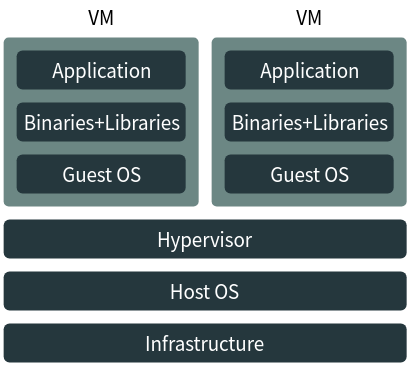
\includegraphics[width=100mm, scale=0.6]{Images/VM_Illustration.png}
      \caption{Components of a Virtualised Environment} 
      \medskip
	  \small
		A conceptual diagram showing the components of a virtualised environment. Original source: Boolean World. \cite{ContainerAndVMImageSource}
\label{fig:VMConceptualDiagram}
\end{figure}

VMs are relatively heavyweight and expensive to maintain, since each separate VM maintains its own operating system (OS) image\footnote{An OS image is system image is a copy of the entire state of an OS stored in a persistent, non-volatile form. It is a package that contains all of the information required to run the OS on the machine, and is usually relatively large as a consequence.}: An overhead in memory and storage footprint. This lack of flexibility also limits the portability of applications that run on virtual machines between different hosting solutions: It is difficult to replicate the same environment configuration on a second VM.

However, VMs allow for multi-tenancy on a single piece of physical hardware, as well as fine-grained resource allocation. 

\subsection{Platform-as-a-Service}
The idea of PaaS is that users are able to focus on running and developing applications instead of managing the infrastructure that supports them. PaaS systems mean that a virtual infrastructure is provided and users can deploy any application on it without needing to worry how resources are allocated to it.


\subsubsection{Containers}
%Containers are disposable, stateless execution environments for applications.
A container is an isolated execution environment defined by a single package that includes everything needed to run it: Code, runtime, system tools, system libraries, settings. They are type of OS-level virtualisation, isolating an application from the host infrastructure on which it is being run: They are almost completely host-agnostic\footnote{Host-agnostic in this context refers to the fact that containers do not have an affinity to any particular host system.}. An application and all of its dependencies can be packaged up in a \textit{container image} that can be published in a \textit{container registry} so that unlimited numbers of users can work in identical application environments.

\begin{figure}[ht]
      \centering
      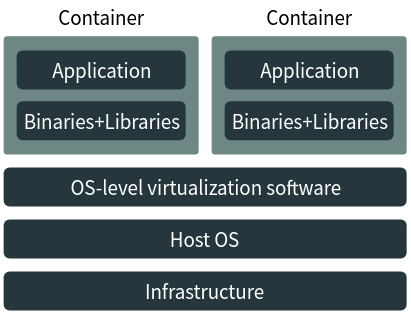
\includegraphics[width=100mm, scale=0.6]{Images/Container_Illustration.png}
      \caption{Components of a Container Environment} 
      \medskip
	  \small
		A conceptual diagram showing the components of a container. Original source: Boolean World. \cite{ContainerAndVMImageSource}
      \label{ContainerConceptualDiagram}
\end{figure}


For setting up a standard application environment and deploying a large number of instances on-demand, containers are simple to configure and much faster to launch than VMs. Among the many advantages of using containers compared to VMs are the following: 
\begin{enumerate}
\item Hosting a container does not include anywhere near the same storage overhead as a VM: Containers do not need to maintain their own copy of the OS image, since they share the kernel of the host OS.
\item All dependencies required by an application are packaged into a single, replicable image. This means that the portability of application environments that is so difficult to achieve with VMs, is native in containers.
\item Containers come with their own separate network stack and storage without the overhead of building and running a VM. 
\end{enumerate}

Many organisations are migrating their infrastructure deployments from VMs to containers. A recent example of this is Netflix, who started migrating their infrastructure hosting to the AWS cloud in 2008. At the time of writing in 2018, Netflix are migrating the hosting of all of their applications from VMs to containers. In a paper discussing this shift in Netflix's infrastructure approach, \cite{NetflixContainerMigration} Leung \textit{et al.} state that ''one of the benefits of using containers ... is that it abstracts much of the machine-centric management that applications were doing in VMs''. This is one of the notable benefits of using containers over VMs: Those deploying the application no longer need to concern themselves with the environment specifics, and get the opportunity to focus on building and running applications.


%\subsubsection{Microservice Architectures}
%Microservice architecture design is an increasingly popular design for distributed systems on all levels, moving away from failure-prone monolithic designs of the past. 


%* granular resource management 
%* loose coupling of services
%* Greater ability to scale

%Microservice architectures also have strengths from a network security perspective by providing air-gapping. An air gap is security measure employed in networks that isolates components of a system from insecure or untrusted components of the system. By isolating functionally separate parts of a system from each other, the number of components of the system immediately affected by a single compromise is minimised and can be confined more easily. From the perspective of performance, it eliminates the possibility of a ''single point of failure'',  reducing the exposure of the overall system to compromise.

\subsubsection{Security through Containerisation} \label{SecurityThroughContainerisation}
%% A lot of this will be covered in the design chapter
An area where much work remains to be done is in bringing security applications into the progressively more popular container ecosystem. There is tremendous potential for the containerisation of security applications, and a number of identified benefits of this approach are described below.

\begin{itemize}
\item \textbf{Disposability}

A major selling point of containers is that they are virtually disposable. In the event that a container becomes infected with malware, it is straightforward to remove it entirely and re-deploy it with minimal disruption to the system. 

\item \textbf{Isolation}

One of the key features of containers which has contributed to their widespread adoption is the ability to restrict and isolate application environments. 

	\begin{itemize}
    \item Containers leverage a Linux functionality known as ''namespaces'', placing applications that run on them in restricted environments, isolated from each other. Individual containers are run in their own independent namespace, and are given their own independent view of a  variety of operating system resources. 

	\item Containers can also be restricted such that any ''root user privileges'' do not have to correspond to the root user privileges on the host machine: The definition of ''root user privileges'' is completely separate from those of the host. 
    
    \end{itemize}
    The net impact of this isolation on the security of containers is that the applications running inside one container will not interact, unless explicitly configured to do so, with applications inside another container or on the host machine. This is a substantial increase in security compared to running multiple non-containerised applications on the same system, and means that even if one container is compromised by malware, the others can continue to operate. This loosely-coupled approach to operating services has the capacity to deliver greater fault tolerance and scalability in systems in which they are deployed, reducing the exposure of the overall system to compromise.
\item \textbf{Standard Base OS Images}

Containerised solutions benefit greatly from being able to build customised containers off standard, widely-used OS images. These standard images benefit from ongoing security auditing and patching, making them a secure foundation for building customised containers. 

\item \textbf{Customisability}

Containers are highly customisable, and enable fine-grained control for system administrators. It is possible to restrict everything from the privileges to the runtime services, enabling restriction of what resources can be accessed by any given container. 

\end{itemize}

In an infrastructure ecosystem where services are increasingly being containerised, the containerisation of security applications is a must in order for them to remain compatible with these new architectures. However, the introduction of new technologies into systems will always bring additional security risks, something that must be carefully considered by organisations migrating their operations to container-based architectures. \cite{7742298} 



%%
%% SECTION 4: CLOSELY RELATED WORK
%%

\section{Closely Related Work} \label{CloselyRelatedWork}


The closely related projects described in this section are explored from the point of view of their most interesting characteristics rather than the achievement of their respective research objectives.
%TODO a little explanation of what the reader should find in this section.


\subsection{Adaptive Honeypots} \label{RelatedHoneypotProjects}

The goals of honeypot deployments can vary greatly, and most honeypots offer a wide variety of options and different functionalities in order to provide flexibility to this end. As identified in \textit{Section \ref{HoneypotDesignSoA}}, increasing the interaction capabilities of a honeypot results in more extensive and detailed information but also more potential damage to the system. Different trade-offs in honeypot design are clearly more suitable for some deployment scenarios than others.

At the time of writing, there were over 1,000 open-source honeypot projects listed publicly on GitHub\footnote{On 24th March 2018, a search for the query 'honeypot' provided 1,405 repositories as results.}. These range from open-sourced production honeypots to major open-source collaborations and hobbyist projects. Research honeypots discussed in journals and conference papers add even more to this number, and there is little doubt that many proprietary production solutions also exist. \cite{CanaryThinkst}

Some of the more significant honeypot projects encountered during this research are described below. These include research honeypots and community-based honeypot developments.% and open-sourced production honeypots.



\subsubsection{Kippo} \label{AboutKippo}
	
	Kippo is an open-source SSH honeypot written in Python which is no longer under active development. It is a medium-interaction honeypot developed by an online development community, and is designed to capture the entire session interaction of an attacker. \cite{KippoHoneypotGithub} It emulates a Debian Linux installation, and provides a wide variety of features as follows:
    
    \begin{itemize}
    \item Kippo provides an out-of-the-box configurable file system and shell for each attacker to interact with. It does not limit the number of simultaneous sessions, and can present a mock file system and shell to each attacker independently.
    \item Kippo implements a falsified SSH service to which attackers can connect.
    \item Kippo includes configuration options for permitted usernames and password combinations which can be controlled by the user.
    \item All interactions with Kippo are logged, including brute-force login attempts, source IP addresses, attacker protocol information, commands executed and records of any attempted downloads.
    \end{itemize}	
	 The fact that Kippo is implemented as a Python application means that attackers will not interact directly with the underlying OS, adding an extra layer of protection for the host system. The fact that it doesn't call on any external software for its core operations makes it much less vulnerable to third-party compromises. 

	Kippo does not have the capability to execute malware, but can be used in conjunction with other solutions such as Cuckoo Sandbox\footnote{Cuckoo Sandbox is an open-source malware analysis system, which allows malicious files to be executed inside an isolated environment in order to analyse their behaviour and properties. \cite{CuckooSandbox}} in order to execute and analyse malware safely in a controlled environment.

Unfortunately, Kippo is an example of a honeypot which is susceptible to fingerprinting due to the fact that it emulates a real system: In its emulation of the OpenSSH service, it is possible to trigger characteristic responses identifying the device as a Kippo honeypot using carefully crafted messages. \cite{Nawrocki2016} This flaw led to the eventual cessation of active development on the honeypot, rendering it largely unusable in the development of new honeypot-based solutions.
	
	\subsubsection{Cowrie} \label{AboutCowrie}
	
	Cowrie is a medium-interaction honeypot which was originally forked from the Kippo project by security researcher Michel Oosterhof. It is actively maintained and supported by a dedicated community, who provide quick response times to queries and bug-fixes. It is widely used in both research and production projects as a medium-interaction honeypot. \cite{PickyAttackers2017} \cite{TPotWebpagev17} \cite{ModernHoneyNetworkLaunchAnnouncement} 
    
	In addition to the capabilities and features provided by the Kippo honeypot, Cowrie has some additional features \cite{CowrieGithub} \cite{CowrieWebsite} including but not limited to the following:
	
	\begin{itemize}
		
		\item Cowrie enables attackers to gain access to the honeypot using an emulated telnet client as well as SSH, supporting the two protocols which are most widely-targeted by IoT botnets. \cite{UnderstandingTheMiraiBotnet} \cite{HajimeMysteriousBotnet}
		
		\item Cowrie logs all attack session information in JSON format, which is a widely-used format that can be processed by many tools;
        
        \item Cowrie provides integration with a number of useful tools including VirusTotal malware database and the Mailoney SMTP honeypot;
        
		\item Cowrie also improves substantially on its predecessor, Kippo, resolving many of the major fingerprinting issues.
	\end{itemize}

    Interestingly, there is also some activity with respect to containerisation of the Cowrie honeypot. A basic Cowrie container image has been developed by contributors to the Cowrie project, \cite{DockerCowrie} which illustrates an increasing awareness of the need to migrate security applications into container-driven architectures.
	
	\subsubsection{Honeyd} \label{AboutHoneyd}
    
    Honeyd is an important predecessor to many of today's honeypots, and is likely the best-known honeypot implementation. It is an open-source, virtualised low-interaction honeypot released originally in 2002, and is currently in maintenance mode. It was originally developed by Niels Provos. 
    
     Honeyd is flexible and adaptive in that it can be configured both to run arbitrary services and to advertise itself as running different operating systems, learning the service ''personalities'' by reading Nmap fingerprint files in order to mimic them. \cite{HoneydWebsite} It cannot however emulate system components such as file systems or command execution. As explained in an article \cite{ProvosHoneyd} by creator Niels Provos, Honeyd ''listens to network requests destined for its configured virtual honeypots'' and ''responds according to the services that run on the virtual honeypot. Before sending a response packet to the network, the packet is modified by Honeyd's personality engine to match the network behaviour of the configured operating system personality.'' 

Additional features of Honeyd include the ability to create virtual routing topologies, and the ability to enhance configured routes with realistic latency and packet loss characteristics in order to appear more convincing. Though it has provided inspiration for finding adaptive solutions for honeypots, the fact that it is no longer being actively developed renders it largely unusable in new deployments.

\subsubsection{IoTPot} \label{AboutIoTPot}
	
	IoTPot is a research honeypot developed by Yin Minn Pa Pa \textit{et al.}, which they describe as ''a novel honeypot that emulates interactions of the telnet protocol and a variety of IoT devices''. \cite{IoTPot2016} It is a reactive IoT honeypot that targets the study of telnet-based attacks.  It is particularly interesting because of its ability to react to the requests sent by attackers, providing them with a dynamically generated response deemed to be most likely to match the CPU architecture of the system that is being targeted in the attack. 
    
\begin{figure}[ht]
      \centering
      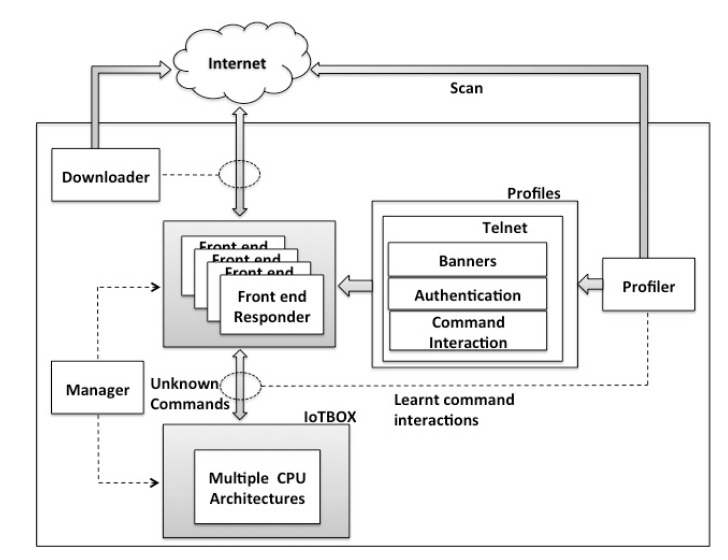
\includegraphics[width=150mm, scale=1]{Images/iot-pot-sys-arch.PNG}
      \caption{The IoTPot Honeypot Architecture} 
      \medskip
	  \small
		This diagram is originally from a paper published by the researchers who developed the IoTPot honeypot, and illustrates the operation of the IoTPot system. \cite{IoTPot2016} 
\label{fig:Images/iot-pot-sys-arch.PNG}
\end{figure}
    
    IoTPot was designed in recognition of the fact that there are too many different types of IoT device to be able to develop honeypots for all of them. The principles behind the operation of IoTPot are very much based on a honeypot network called SGNET, where low-interaction sensors forward attacks that they receive to a high-interaction honeypot to handle. \cite{SGNET} This is similar to the function of the \textit{front-end responder} in IoTPot, which is the component of the system that interacts directly with attackers. A diagram of the system architecture can be seen in figure \ref{fig:Images/iot-pot-sys-arch.PNG}.
    
    \begin{itemize}
    \item The \textit{front-end responder} component deals with negotiating the Telnet protocol with an attacker based on what it believes they are looking for. It emulates a number of different device profiles, and for each device profile deals with authentication attempts, command interactions and emulation of device-specific telnet options.
\item If a command is issued by the attacker that the \textit{front-end responder} doesn't know how to handle, it connects via Telnet to the \textit{back-end responder}, a component called \textit{IoTBox}. This component contains emulated operating systems for a number of different CPU architectures, meaning that the command can be executed on each of these and an appropriate response returned to the attacker as a result.
    \end{itemize}
     
    Most honeypots are far more passive in their approach to handling incoming commands from attackers, and are incapable of providing any more than one valid response to a given request. At the time that it was developed, the researchers claimed that there existed no other IoT honeypot ''that can mimic IoT devices of many different CPU architecture while listening on 23/TCP with the ability to learn unknown command interactions.'' 
    
    As an adaptive telnet honeypot, IoTPot appears to be very effective. However, it is relatively restricted in that it can only deal with telnet-based attacks, limiting the attacks it can capture. According to the paper, the researchers ''plan to extend IoTPot to support more protocols that are likely the target of attacks'' in the future.

	
	\subsubsection{IoTCandyJar} \label{AboutIoTCandyJar}
IoTCandyJar is a recent IoT honeypot developed by Luo \textit{et al.} who classify it as an \textit{intelligent-interaction} honeypot rather than as low, medium or high-interaction. \cite{IoTCandyJar} The researchers explain that ''the goal of intelligent interaction is to learn the 'correct' behaviors to interact with clients from zero knowledge about IoT devices''. Their approach is to utilise machine learning techniques to determine the most appropriate tactics to prolong attacks.

The IoTCandyJar honeypot is composed of a number of primary modules, which can be seen in figure \ref{fig:Images/iot-candy-jar-sys-arch1.PNG} as follows:
\begin{itemize}
        \item The \textit{IoTScanner} module leverages the fact that there are powerful scanning tools freely available to identify IoT devices, using \textit{Shodan, Censys, Masscan} and \textit{Zoomeye} scanning tools to identify IoT devices on the internet. It actively probes these devices, collecting their responses to various requests that have previously been captured by IoTCandyJar. 

        \item The \textit{IoTLearner} module builds intelligence into the honeypot, using the responses captured by the \textit{IoTScanner} module to train a model using machine learning algorithms. The accuracy of the responses provided to requests improve with increasing numbers of interactions with attackers: If an attacker sends a second request after receiving a response from IoTCandyJar, the response is deemed to have been correct.

      \item The \textit{IoTDatabase} stores all of the captured requests and responses, and stores any information relating to the machine learning model.
\end{itemize}    

\begin{figure}[ht]
      \centering
      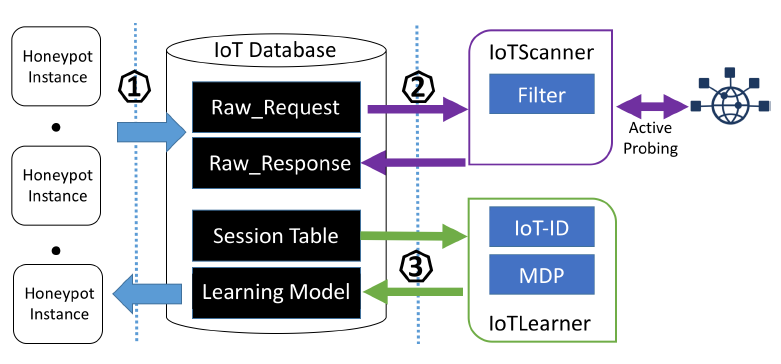
\includegraphics[width=150mm, scale=1]{Images/iot-candy-jar-sys-arch1.PNG}
      \caption{The IoTCandyJar Honeypot Architecture} 
      \medskip
	  \small
		This diagram is originally from a paper published by the researchers who developed the IoTCandyJar honeypot, and illustrates the operation of the IoTCandyJar system. \cite{IoTCandyJar} 
\label{fig:Images/iot-candy-jar-sys-arch1.PNG}
\end{figure}

The major selling point of IoTCandyJar is the dynamic approach that it takes to reacting to probing by IoT botnets. Similarly to IoTPot, IoTCandyJar aims to provide the best response to an attacker based on what they are determined to be seeking. The major difference between these two honeypots is in the approach they take to achiev this: Where IoTPot determines the most appropriate response by generating the correct response through execution of the request, IoTCandyJar learns the best response to a request based on interacting with attackers. Responses to attacker requests are generated based purely on what the system has learned from previous interactions with attackers, and not through any execution of requests. \cite{IoTCandyJar}

    
  	\subsubsection{Zigbee Honeypot} \label{AboutZigbeeHoneypot}
    Dowling \textit{et al.} developed a research honeypot targeted at attackers of Zigbee devices, which are devices commonly used in WSNs. \cite{Dowling2017} The development of this honeypot was motivated by the fact that as these IoT devices are being more widely-deployed and their vulnerabilities are also becoming well understood: Therefore, an assessment of the threat to these devices is essential.
      
    In their implementation of the honeypot, Dowling \textit{et al.} included a number of interesting measures to initiate the interest of attackers in the honeypot:
    
    \begin{itemize}
    \item The host name for the honeypot was configured to be \textit{zigbee-gateway} as a means of assessing whether there is any awareness of Zigbee devices amongst attackers;
    \item The researchers implemented a means of transmitting of fictitious medical traffic, which is transmitted in cleartext over an unfiltered network. 
    \end{itemize}
    
    The generation of potentially interesting network traffic in order to entice attackers to attack the honeypot is a thought-provoking feature of this solution. Though the research conducted is largely focused on identifying whether there is any awareness of Zigbee devices specifically, the idea of adapting the honeypot to the attackers it wishes to attract is a useful one.   
  

\subsection{Containerised Honeypots} \label{RelatedHoneynetProjects}
Related projects identified in the domain of containerisation of honeypots are limited in number, primarily because the security domain is still catching up with the migration of infrastructures to container-based architectures. The research conducted in these related projects focus on both the benefits of using containers for hosting honeypots, and the challenges that are faced in doing so.

	\subsubsection{Distributed Virtual Honeynets} \label{AboutDistributedVirtualHoneynets} 
    In 2014, Pisarcik \textit{et al.} developed a distributed honeynet of high-interaction honeypots using containers for OS-level virtualisation, an approach which at the time was relatively unexplored in research. \cite{Pisarcik:2014:FDV:2659651.2659685} Their motivations for developing such a solution were:
    \begin{itemize}
    \item The fact that administering honeypot-driven systems is time-consuming, motivating the use of containers to simplify their management; and
    \item The ability of honeypots to correlate attack events in order to determine whether they are localised or distributed in nature, quickly allowing for identification of attack trends.
    \end{itemize}
    
    Though the approach to designing and evaluating their honeynet solution is worthy of note, the more significant contribution made by this research is in relation to the containerisation of honeypots and honeynets. The research highlights that when compared to virtual machines or bare-metal systems, OS-level virtualisation incurs very little performance or maintenance overhead. \cite{Pisarcik:2014:FDV:2659651.2659685} As well as this, they note that using containers adds an additional layer of deception to honeypots: Since they are isolated environments sharing the kernel of a real OS, they are more likely to appear as a legitimate system when fingerprinted. 
    
    All of these features would make it seem that containers are a perfect deployment solution for honeypots: However, they also address the potential security pitfalls of using containers to host honeypots, particularly because of the risk to the host system by virtue of sharing its OS kernel with containers. These are interesting insights regarding the practicality of using containers in honeypot-driven solutions.

   
    \subsubsection{Using Linux Containers for Deceptive Honeypots} \label{AboutDeceptiveHoneypots}
    In a paper published in 2017, Kedrowitsch \textit{et al.} explore the use of Linux-based containers (LXCs) in honeypot deployments. \cite{LXCsForDeceptiveHoneypots2017} However, the use of LXCs here is examined from the perspective of their ability to evade detection by malware, which has often been found to change its behaviour after detecting a VM-based environment. \cite{SpotlessSandboxes} The motivation behind this is to identify whether container environments will be feasible in the long term as an approach to hosting honeypots without being detected by malware.

The researchers performed a number of experiments where they compared the fingerprinting weaknesses of LXCs to those of bare-metal systems and VMs. They focused on the typical techniques that malware employs in fingerprinting VMs: Comparing the response generated for a particular input against the response that would be expected from a bare-metal system. In particular, they chose to test and compare the following properties of VMs and containers as a means of fingerprinting:

\begin{itemize}
    \item Variability and execution time in CPU clock sampling;
    \item Reported CPU information;
    \item Instruction execution time.
\end{itemize}

When evaluating their experiments, it was found that containers were much less susceptible to fingerprinting than their VM counterparts, which was expected due to the fact that LXCs are executed directly on bare-metal hardware as isolated processes whereas VMs are not. However, it was strongly concluded that if a malware author wanted to detect a container environment as a means of fingerprinting a system, they would have no difficulty in doing so. 
    

\subsection{Honeypot-Driven Cyber-Incident Monitors} \label{RelatedIncidentMonitorProjects}
Projects listed in this section are relevant since they make the use of honeypots much more accessible to individuals and organisations. They recognise the importance of data aggregation and visualisation from multiple honeypots in order to provide important data to key decision makers, encouraging the use of active network defence by making it much easier to manage and benefit from.

	\subsubsection{TraCINg} \label{AboutTraCINg}
    
    TraCINg is a honeypot-driven cyber incident monitor developed by academic researchers Vasilomanolakis \textit{et al.} in 2015, \cite{Vasilomanolakis}. Its development was motivated by the observation that the consolidation of data gathered from honeypots in different deployment contexts can allow attack data to be correlated, enabling the identification of emerging outbreaks of related attacks. 
    
    The TraCINg system gathers data from a large number geographically distributed honeypots with the aim of correlating attack events. Many of these honeypots are deployed on cloud platforms, which was the approach determined by the researchers to provide the greatest diversity of deployment locations and maximum system uptime for uninterrupted monitoring. Arbitrary open-source honeypots can be used with the TraCINg system, provided that their data is logged in JSON format.
    
   This incident monitoring solution is not intended to be highly deployable or low-cost for use in production systems, but addresses the consideration of aggregating and summarising complex data in a meaningful manner through visualisation, enabling the succinct description of important data for key decision-makers. Their proposal for correlation of data from large deployments distributed honeypots is very interesting: However, their solution uses two low-interaction honeypots, limiting the level of detail of the attack data captured. An improved system would be able to capture more data about attack events in order to gain greater insights into the motivations and methods of attackers.

  
    \subsubsection{TPot} \label{AboutTPot}
    The TPot project is a honeypot-based incident monitor that was developed by Deutsche Telekom, and which they use in their production networks for early threat detection. They decided to open-source their development with the aim of making the deployment of honeypots in production networks more feasible for organisations. \cite{TPotWebpagev17}
    
    TPot supports multiple open-source honeypots hosted in containers. The system consists of a number of components, the most relevant of which are listed as follows:
    \begin{itemize}
    \item \textbf{Containerised Honeypots}

	The TPot system leverages the benefits of containers listed in \textit{Section \ref{SecurityThroughContainerisation}} in order to provide a highly deployable honeypot system. The containerised honeypots supported by the TPot platform are all actively maintained and target a variety of different interactivity levels and attackers\footnote{The honeypots supported by the TPot platform at the time of writing are Conpot, Cowrie, Dionaea, Elasticpot, eMobility, Glastopf, Honeytrap, Mailoney, rdpy and VNClowpot. \cite{TPotWebpagev17}}.

        \item \textbf{The ELK Stack}
    
    The Elasticsearch-Logstash-Kibana (ELK) stack is a collection of log management tools that perform search, logging and visualisation functions respectively. In TPot they are used to analyse, index and represent logged attack data captured by the honeypots.

    \end{itemize}
    
    \begin{figure}[ht]
      \centering
      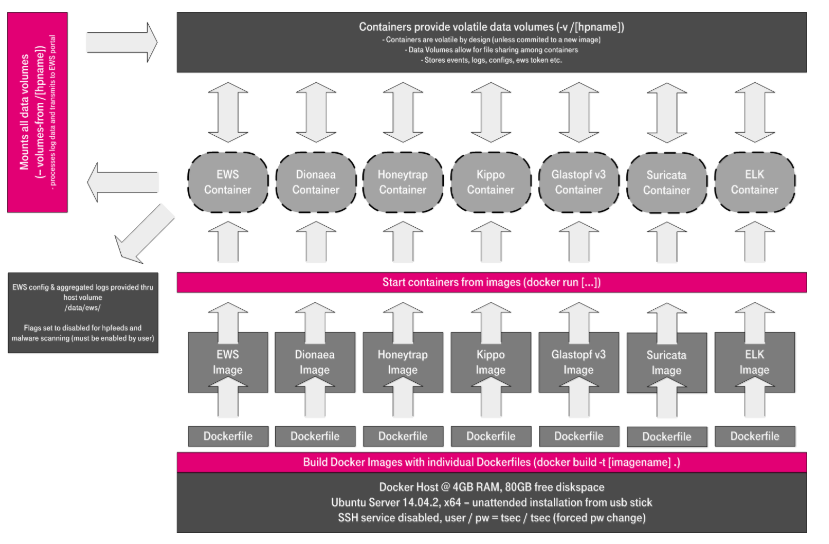
\includegraphics[width=160mm, scale=1]{Images/t-pot-diagram.PNG}
      \caption{Diagram of the TPot Architecture} 
      \medskip
	  \small
		This diagram is provided by the developers of the TPot project as an explanation of the operation of the system. \cite{TPotWebpagev16} Each honeypot is defined by a \textit{Dockerfile}, which is built into an \textit{image}. This image is then used to run the honeypot, and data generated by the honeypot is stored in volumes shared with the host system. The data can then be passed to other systems such as Deutsche Telekom's in-house data aggregation tool \textit{EWSPoster} as shown. 
\label{fig:Images/t-pot-diagram.PNG}
\end{figure}
    
    An infographic provided by the TPot developers can be seen in figure \ref{fig:Images/t-pot-diagram.PNG}. All container images for the honeypots are built based on the Alpine Linux\footnote{Alpine Linux describes itself as a security-oriented, lightweight Linux distribution based on \textit{musl}, \textit{libc} and \textit{busybox}.} container image, which has a particularly small image size meaning that its storage footprint is minuscule. A benefit of running the honeypots inside containers that the developers highlight on their webpage is that they can ''run multiple honeypot daemons on the same network interface while maintaining a small footprint and constrain each honeypot within its own environment''. \cite{TPotWebpagev16}

The proposition of leveraging the benefits of containers in order to host honeypots is an intriguing one, particularly since the difficulties of deploying and maintaining honeypots have been a huge barrier to their widespread adoption to-date. The work on this project by Deutsche Telekom strengthens the case for the coupling of containerised honeypot deployments and visualisation tools.
    
    \subsubsection{Modern Honey Network} \label{AboutMHN}
    The Modern Honey Network (MHN) is a production system developed by Anomali Inc. to manage enterprise honeypot deployments. Their decision to open-source the system was motivated by similar reasons as those given by the TPot developers, being that the deployment and maintenance of honeypot deployments has always been ''a complicated process reserved for security companies and security researchers.'' \cite{ModernHoneyNetworkLaunchAnnouncement} The result is that the MHN simplifies the process of deployment and management of honeypots, making it more feasible for organisations to use active network defence.
    
    The MHN is a centralised server system which is concerned with managing the deployment of honeypots as well as the aggregation of their data. It has support for a large number of open-source honeypots, including the Cowrie honeypot\footnote{The full list of supported honeypots is as follows: Amun, Cowrie, Conpot, Dionaea, ElasticHoney, Glastopf, Shockpot, and Wordpot. MHN also supports threat detection tools including Snort, Suricata and p0f.}. All of these honeypots are low or medium interaction open-source honeypots, which the MHN team say were selected to minimise the risk associated with a deployment of honeypots in a production environment. Honeypot data collected by the MHN system can be visualised with Splunk, a data analysis and visualisation tool: However, unlike TPot's support for the ELK stack, Splunk is not shipped as part of the MHN system.

    
\section{Summary} \label{SoASummary}
Based on the background provided in this section, it is obvious that the field of cybersecurity is dynamic and full of challenges. As aptly phrased by Fred Schneider, ''like good health, cybersecurity is never going to be a \textit{solved problem}''. 

Many of these challenges are the result of gross negligence on the part of manufacturers and system designers; Others are due to obvious oversights and mistakes resulting from a lack of usability; Yet others are a consequence of not understanding the implications that insecure technologies can have for privacy and safety. What all of these present is an opportunity for improvement of current approaches to the implementation of technologies and connected systems.

The work done by those researchers and developers behind the \textit{closely related projects} described in \textit{Section \ref{CloselyRelatedWork}} indicates the awareness and interest that exists around tackling the challenges that are being faced in the security of modern systems. It is a similar interest and awareness on the part of the author which motivates the decision to improve on the current state of the art in this area.

